\chapter{Aufbau und Analyse der ETL-Prozesse}

\section{Überblick über die verwendeten Datenquellen}
Eine der Anforderungen an die Web-Applikation ist den Nutzern aktuelle
Informationen über die Wetter- und die Wellenverhältnisse in den
nächsten Tagen zu bieten. Hierfür werden die frei erhältlichen
Ergebnisse von zwei numerischen Wettermodellen verwendet, dem
\textit{Global Forecast System} und dem \textit{Wave Watch III}
Modell. Bevor diese beiden Wettermodelle näher beschrieben werden und
wie auf die Ergebnisse der Modellberechnungen zugegriffen werden kann,
wird zunächst kurz erklärt, wie heutige Wettervorhersagen zustande
kommen und welche Rolle dabei numerische Wettermodelle spielen.

\subsection{Wettervorhersagen}
Wettervorhersagen haben das Ziel, den Zustand der Erdatmosphäre zu
einer bestimmten Zeit an einem bestimmten Ort zu prognostizieren. Sie
werden meist von staatlichen aber auch privaten Wetterdiensten
erstellt, die sich den Erkenntnissen der Meteorologie
bedienen. Heutige Wettervorhersagen basieren auf den aufwändig
berechneten Ergebnissen numerischer Wettermodelle.

Die Vorhersage des Wetters ist ein Anfangswertproblem, das meist in
drei Schritten gelöst wird. Im ersten Schritt, der Analyse, wird der
Ausgangszustand der Atmosphäre bestimmt. Dieser Zustand wird durch
verschiedene physikalische Größen festgelegt, die von Wetterstationen,
Satelliten, Bojen oder Flugzeugen gemessen werden. Einige typische
Größen sind Luftdruck, Temperatur, Wind, Wasserdampf, Wolken und
Niederschlag.

Die Modellberechnung ist der zweite Schritt. Mit ihr wird die
zukünftige Entwicklung der Atmosphäre in Form der physikalischen
Größen simuliert. Die Berechnung dieser Simulation ist sehr aufwändig
und wird deshalb mit Hilfe von Supercomputern durchgeführt. Ergebnis
der Modellberechnung ist der Zustand der Atmosphäre zu verschiedenen
Zeitpunkten in der Zukunft, dargestellt durch die physikalischen
Größen.

Im letzten Schritt, der Nachbereitung, werden die Ergebnisse der
Simulation schließlich für die verschiedensten Nutzer
aufbereitet. Dies beinhaltet die Generierung von Wetterkarten und
Strömungsfilmen für das Fernsehen, das Erstellen von Warnhinweisen für
Technisches Hilfswerk und Feuerwehr oder die Interpretation und
Analyse verschiedenster Wetterphänomene.

\subsection{Nummerische Wettermodelle}
Numerische Wettermodelle versuchen, den Zustand der Erdatmosphäre und
deren Veränderung im Laufe der Zeit als mathematisches Problem zu
beschreiben. Dabei werden die physikalischen Größen und Beziehungen,
die den Zustand und die Veränderung der Atmosphäre beschreiben, als
System partieller Differentialgleichungen modelliert. Die meisten
Modelle verwenden dabei dieselben physikalischen Gesetzmäßigkeiten,
die auf den Erhaltungssätzen von Energie, Impuls und Masse
beruhen. Meist unterscheiden sie sich aber in der konkreten
mathematischen Formulierung und der numerischen Lösung der
Gleichungssysteme, weshalb die Ergebnisse verschiedener Modelle
voneinander abweichen können.

\subsubsection{Operative Wettermodelle}
Der Deutsche Wetterdienst betreibt drei verschiedene
Wettermodelle. Die lokalen \textit{COSMO-DE} und \textit{COSMO-EU}
Modelle \footnote{COSMO - Consortium for Small-Scale Modelling}
\nomenclature{COSMO}{Consortium for Small-Scale Modelling} liefern
Vorhersagen für Deutschland und Europa, das globale Modell
\textit{GME} \footnote{Global Model} \nomenclature{GME}{Globales
  Modell des Deutsche Wetterdienst} Vorhersagen für die ganze
Welt. Weitere bekannte Modelle sind das von der US-amerikanischen
\textit{National Oceanic and Atmospheric Administration (NOAA)}
betriebene \textit{Global Forecast System (GFS)}
\nomenclature{GFS}{Global Forecast System} und das neuere
\textit{Weather Research and Forecasting (WRF)}
\nomenclature{WRF}{Weather Research and Forecasting} Modell, das vom
\textit{National Weather Service (NWS)} \nomenclature{NWS}{National
  Weather Service}, vom amerikanischen Militär und einigen privaten
meteorologischen Organisationen verwendet wird.

\subsubsection{Diskretisierung von Raum und Zeit}

Um die sich verändernde Atmosphäre der Erde auf ein Modell abbilden zu
können wird eine Diskretisierung von Raum und Zeit vorgenommen. Dabei
wird die Oberfläche der Erde mit einem aus Drei- oder Vierecken
bestehenden Gitternetz überzogen, und die Atmosphäre vertikal in
mehrere Luftschichten aufgeteilt. Damit werden die möglichen
Vorhersagepunkte in der Atmosphäre auf die endliche Zahl der so
entstandenen Kreuzungspunkte reduziert. In Abbildung \ref{gitternetz}
ist das dreieckige Gitternetz des zur Zeit vom Deutschen Wetterdienst
und des Max-Planck-Instituts für Meteorologie neu entwickelten
\textit{ICON} \footnote{Icosahedral Non-hydrostatic General
  Circulation Model} \nomenclature{ICON}{Icosahedral Non-hydrostatic
  General Circulation Model} Wettermodells zu sehen. Das
\textit{Global Forecast System} und das \textit{Wave Watch III} Modell
verwendet ein aus Vierecken bestehendes Gitternetz.

\begin{figure}[h]
  \begin{center}
    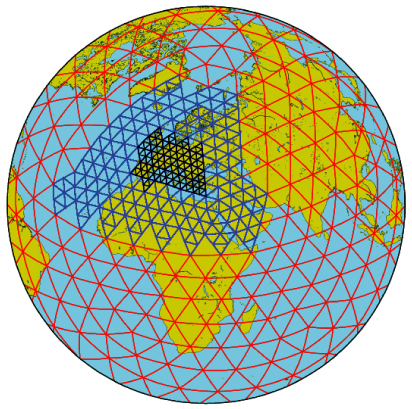
\includegraphics[height=200px]{bilder/gitternetz}
    \caption{Dreiecksgitter des \textit{ICON} Wettermodells (Quelle:
      Deutscher Wetterdienst)}
    \label{gitternetz}
  \end{center}
\end{figure}

Mit der Maschenweite bezeichnet man den Abstand zwischen zwei
benachbarten Gitterpunkten. Je feiner das Gitter bzw. je höher die
Auflösung des Modells ist, desto genauer können die Erdoberfläche und
die darüber liegenden atmosphärischen Strukturen erfasst werden, was
sich wiederum auf die Genauigkeit der Wettervorhersage auswirkt. Die
benötigten Ressourcen zur Berechnung der Modellgleichungen steigt mit
der Anzahl der verwendeten Gitterpunkte.

Da eine sehr hohe Auflösung selbst die Leistungsfähigkeit der
schnellsten Supercomputer übersteigt, werden von den Wetterdiensten
meist verschiedene Modelle in unterschiedlichen Auflösungen
berechnet. Globale Modelle, die den gesamten Globus umfassen, werden
mit einer geringeren Auflösung berechnet als lokale Modelle, die nur
einzelne Länder oder Kontinente abdecken. Je weiter aber in die
Zukunft prognostiziert wird, desto mehr spielen aber wieder
Wetterphänomene aus Gebieten, die nicht vom lokalen Modell abgedeckt
werden eine Rolle. Für Vorhersagen ab 5 Tagen in die Zukunft benötigen
die lokalen Modelle wiederum Informationen aus der gesamten
Atmosphäre. Deshalb verwenden die höher auflösenden lokalen Modelle
oft Informationen als Randwerte aus einem zuvor berechneten globalen
Modell.

Die zeitliche Diskretisierung hingegen ist weniger problematisch. Die
meisten Modelle bieten mindestens Prognosen um 12.00 und 24.00 Uhr für
diejenigen Tage an, über die sich der Vorhersagezeitraum
erstreckt. Das \textit{Global Forecast System} und das \textit{Wave
  Watch III} Modell bieten Vorhersagen im drei Stunden-Intervall an,
das lokale \textit{COSMO-DE} Modell sogar in einem Intervall von 25
Sekunden.

\subsubsection{Rechenaufwand heutiger Modelle}

In einer Präsentation
\footnote{\url{http://www.initiative-wissenschaftsjournalismus.de/fileadmin/Downloads/WissensWerte2008/B3_Majewski.pdf}}
aus dem November 2008 wurde der Rechenaufwand für die vom Deutschen
Wetterdienst betriebenen Modelle mit den dazugehörigen Kenngrößen
veröffentlicht. Damals wurden die Wettervorhersagen auf einem IBM
Power 5 System (p575) mit 52 Knoten, 416 Prozessoren und einer
Spitzenleistung von 3,1 Teraflop/s berechnet.

\begin{itemize}
\item Für Deutschland wird das \textit{COSMO-DE} Modell mit einer
  Maschenweite von 2,8 Kilometern betrieben und besteht aus ca. 10
  Millionen Gitterpunkten. Die Berechnung dauert 30 Minuten und
  liefert Vorhersagen in einem 25 Sekunden Intervall für einen
  21-stündigen Vorhersagezeitraum.
\item Das Europa umfassende Modell \textit{COSMO-EU} hat eine
  Maschenweite von 7 Kilometern, ca. 17 Millionen Gitterpunkten und
  wird mit einem Zeitintervall von 40 Sekunden erstellt. Die
  Berechnung einer 24-stündigen Vorhersage dauert 25 Minuten.
\item Das globale, die gesamte Welt umfassende \textit{GME} Modell hat
  eine Maschenweite von 40 Kilometern mit ca. 15 Millionen
  Gitterpunkten. Die Berechnung der 24-stündigen Vorhersage mit einem
  Zeitintervall von 133 Sekunden benötigt 15 Minuten.
\end{itemize}

Leider wurden während der Recherche keine genaueren Informationen
gefunden, wie sich die Berechnung der hier erwähnten Modelle auf dem
seit März 2009 beim Deutschen Wetterdienst in Betrieb genommenen
Vektorsupercomputer SX-9 der Firma NEC verhält. Die Spitzenleistung
dieses Systems beträgt momentan 4,5 Teraflop/s, die bis 2010 auf 11
Teraflop/s aufgestockt werden soll. Mit dieser neuen Anschaffung will
der Deutsche Wetterdienst unter anderem auch Wettervorhersagen mit
einer Auflösung von 2,8 Kilometern für Deutschlands Anrainerstaaten
berechnen.

\subsection{Geographische Breite und Länge}
Zur Festlegung von Punkten auf der Erde wird meist ein
Koordinatensystem genutzt, dessen Grundlage parallel zum Äquator
verlaufende Breitenkreise und die beiden Pole verbindende
Längenhalbkreise sind. Der am Äquator angesiedelte Breitenkreis teilt
die Erde in die nördliche und die südliche Halbkugel. Sowohl auf dem
nördlichen als auch auf dem südlichen Teil verlaufen jeweils weitere
90 Kreise, den Äquator mit eingeschlossen, also insgesamt 181
Breitenkreise. Die beiden Pole werden durch 360 nebeneinander liegende
Längenhalbkreise verbunden, von denen der durch die Sternwarte in
\textit{Greenwich} verlaufende Halbkreis als Nullmeridian bezeichnet
wird. Die Zählung fängt am Nullmeridian an, und geht jeweils um 180
Schritte in beide Richtungen. Nullpunkt des Koordinatensystems ist
derjenige Punkt, an dem der Nullmeridian den Äquator kreuzt. In
Abbildung \ref{koordinaten} ist der durch \textit{Greenwich} laufende
Nullmeridian und der 30 $^\circ$ nördlich verlaufende Breitenkreis zu
sehen.

\begin{figure}[h]
  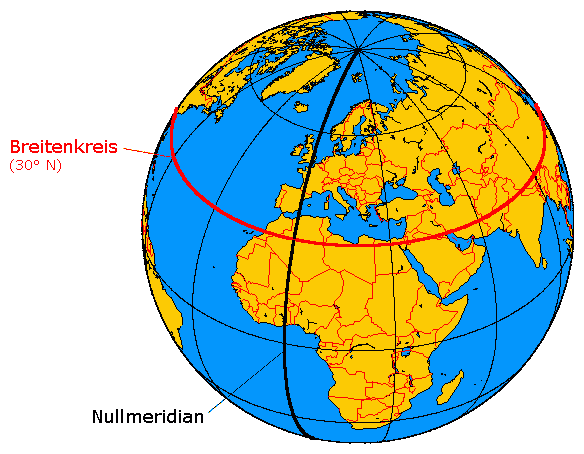
\includegraphics[width=310px]{bilder/koordinaten}
  \caption{Die in Breiten- und Längenkreise unterteilte Erdkugel (Quelle: Wikipedia)}
  \label{koordinaten}
\end{figure}

Die Position eines Punktes auf der Erde wird durch seine geographische
Breite (\textit{Latitude}) und Länge (\textit{Longitude})
angegeben. Dies sind die in der Einheit Grad angegebenen, und vom
Nullpunkt aus gesehenen Abstände der durch diesen Punkt verlaufenden
Breiten- und Längenkreise. Die Position von \textit{Greenwich} ist
beispielsweise durch die Angabe \textit{51.479 $^\circ$ N, 0.0
  $^\circ$ E} festgelegt.


\subsection{Angaben zur Modellauflösung}
Das \textit{Global Forecast System} und das \textit{Wave Watch III}
Modell beziehen sich ebenfalls auf dieses Koordinatensystem, und deren
Gitterauflösung wird in der Einheit Grad angegeben. Da die meisten
Menschen aber bei Distanzangaben in einer Längeneinheit denken an die
sie gewöhnt sind und unter der sie sich auch etwas vorstellen können,
stellt sich die Frage, wie viele Kilometer bzw. Meilen der Abstand
zwischen zwei Knotenpunkten des Gitternetzes beträgt.

Aufgrund der elipsoiden Gestalt der Erdkugel kann hierzu jedoch keine
allgemeingültige Aussage getroffen werden, da dies von der jeweils
betrachteten Region auf der Erdkugel und dem verwendeten
Referenzellipsoiden abhängig ist. Ein Breitengrad (\textit{Latitude})
entspricht durchschnittlich etwa 111 Kilometern und ist weitestgehend
konstant. Der Abstand zwischen den Längengraden (\textit{Longitude})
variiert allerdings erheblich. Am Äquator beträgt dieser Abstand
ebenfalls ungefähr 111 Kilometer, konvergiert aber an den Polen in
Richtung Null. Die hier teilweise in Kilometern angegebenen
Gitterauflösungen sind demnach nur als grobe Richtwerte zur besseren
Einschätzung der Gitterauflösung zu verstehen und beziehen sich auf
die Regionen um den Äquator. Eine praktische Zusammenfassungen mit
Formeln zur Berechnung von Problemen aus dem geographischen Bereich
sind unter \cite{aviation} und \cite{movable_type_scripts} zu finden.

\subsection{Global Forecast System}
Das \textit{Global Forecast System} ist ein globales numerisches
Wettermodell, das vom \textit{National Weather Service} betrieben wird
und den gesamten Erdball abdeckt. Da die Ergebnisse der
Modellberechnung über das Internet
\footnote{\url{http://nomad5.ncep.noaa.gov/pub/gfs}} erhältlich sind
und von jedem verwendet werden dürfen, erfreut es sich einer großen
Beliebtheit. Das Modell liefert Vorhersagen bis zu 384 Stunden (16
Tage) in die Zukunft und wird mit variierenden Auflösungen viermal
täglich berechnet, jeweils um 6.00, 12.00 und 18.00 und 24.00 Uhr
koordinierter Weltzeit (\textit{UTC}). Die ersten 180 Stunden werden
mit einer Maschenweite von ca. 40 Kilometern und einem Intervall von 3
Stunden berechnet, die restlichen Stunden im 12-Stunden-Intervall und
einer Auflösung von ca. 80 Kilometern. Vertikal wird die Atmosphäre
bei beiden Auflösungen in 64 unterschiedliche Luftschichten
aufgeteilt.

Das Modell berechnet eine Vielzahl von physikalischen Größen, von
denen hier hauptsächlich die Temperatur, die Gesamtbewölkung und das
Niederschlagswasser von Bedeutung sind. Da weithin Einverständnis
darüber herrscht, dass Vorhersagen über 180 Stunden hinaus sehr
ungenau sind, verwenden die hier entwickelten \textit{ETL} Prozesse
nur die ersten 180 Stunden in der höchsten Auflösung.

\subsection{Wave Watch III}
Um für mehr Sicherheit auf hoher See und an Küstenregionen zu sorgen,
betreibt der \textit{National Weather Service} das \textit{Wave Watch
  III} Wettermodell, um Wellen vorherzusagen. Es liefert
ausschließlich Informationen über diejenigen Wellen, die durch den
direkten Einfluss von Winden entstehen. Wellen, die durch andere
Ereignisse wie z.B. Gewitter, Gezeiten oder Tsunamis verursacht
werden, sind in diesem Modell nicht berücksichtigt. Da sich Wellen
viel zu sehr voneinander unterscheiden, werden nicht Vorhersagen für
einzelne Wellen getroffen, sondern über die Statistik von mehreren
Wellen. Das Modell liefert sowohl Informationen über die Wellenhöhe,
die Wellenperiode und die Wellenrichtung als auch über die Windstärke
und die Windrichtung.

Das Modell wird wie das \textit{Global Forecast System} viermal
täglich neu berechnet und liefert Vorhersagen im 3-Stunden-Intervall
für 180 Stunden in die Zukunft. Die Ergebnisse sind ebenfalls frei
erhältlich
\footnote{\url{http://polar.ncep.noaa.gov/waves/index2.shtml}}. Das
globale Modell wird mit einer Maschenweite von ca. 80 Kilometern
berechnet, die lokalen Modelle mit einer Maschenweite von bis zu 20
Kilometern. Die hier entwickelten \textit{ETL} Prozesse verarbeiten
bisher nur die Daten des globalen Modells. Die Integration der lokalen
Modelle ist für eine der nächsten Versionen der Web-Applikation
geplant, um insbesondere in den Küstenregionen bessere Ergebnisse
anbieten zu können.

\section{Das Gridded Binary Datenformat}
Die Abkürzung \textit{Grib} \nomenclature{GRIB}{Gridded Binary} steht
für \textit{GRIdded Binary} und ist ein bitorientiertes Datenformat
zum Speichern und Übertragen von Wetterdaten. Das Format wurde von der
\textit{Kommission für Basissysteme} (\textit{CBS})
\nomenclature{CBS}{Commission for Basic Systems} der
\textit{Weltorganisation für Meteorologie} (\textit{WMO})
\nomenclature{WMO}{World Meteorological Organization} standardisiert
\footnote{\url{http://www.wmo.int/pages/prog/www/WMOCodes/Guides/GRIB/GRIB1-Contents.html}}
und wird von vielen Wetterorganisationen dazu verwendet die Ergebnisse
ihrer Modellberechnungen kompakt und plattformunabhängig zu speichern
und auszutauschen. Insgesamt wurden drei verschiedene Versionen
spezifiziert, von denen sich mittlerweile die Versionen 1 und 2
etabliert haben. Die mit der Nummer 0 bezeichnete Version gilt als
veraltet und befindet sich bei den meisten Wetterorganisationen nicht
mehr im operativen Einsatz.

\subsection{Struktur von Grib-Dateien}
Eine \textit{Grib}-Datei besteht aus eigenständigen, sich selbst
beschreibenden Datensätzen, den sogenannten \textit{Grib}
Nachrichten. Eine Nachricht enthält dabei alle Daten eines bestimmten
Vorhersageelements, für eine auf ein Gitternetz diskretisierte
geographische Region zu einem bestimmten Zeitpunkt oder
Zeitraum. Beispielsweise die Temperaturen um 12.00 Uhr mittags der
gesamten Erdkugel aus dem \textit{Global Forecast System} oder die
signifikanten Wellenhöhen des \textit{Wave Watch III} Modells für
einen Zeitraum von einer Woche für Europa.

Eine \textit{Grib}-Nachricht besteht wiederum aus mehreren Sektionen,
die den Inhalt einer Nachricht genauer beschreiben und in Tabelle
\ref{tab:grib} aufgelistet sind. Die Sektionen enthalten neben den
eigentlichen Daten Informationen über die Dimension und Auflösung des
verwendeten Gitternetzes, die Herkunft der Daten, die Art des
verwendeten Komprimierungsverfahrens und die physikalische Einheit, in
der die Daten gespeichert sind. \textit{Grib}-Nachrichten können
beliebig oft aneinander gereiht werden, was eine individuelle
Komposition von unterschiedlichen Nachrichten in einer Datei
erlaubt. Dies wird in Abschnitt \ref{subsec:download} ausgenutzt, um
nur ausgewählte Nachrichten aus einer größeren \textit{Grib}-Datei zu
beziehen.

\begin{table*}
  \centering
  {\sf
    \footnotesize
    \begin{longtable}{@{}lp{10cm}@{}}

      \toprule
      \textbf{Name der Sektion} & \textbf{Verwendungszweck} \\

      \midrule
      Indicator & Die Zeichenkette ''GRIB'', Versionsnummer, Länge der gesamten Nachricht \\

      Identification & Charakteristiken, die auf alle Daten zutreffen, u.a. Herkunft der Daten, Referenzzeit und Typ des Produkts \\

      Local Use (optional) & Abschnitt für beliebige zusätzliche Informationen \\

      Grid Definition &  Definition des Gitternetzes, u.a. die Dimension, die Anzahl der Datenpunkte und die verwendete Koordinatenprojektion \\

      Product Definition &  Beschreibung der Daten, Temperatur, Wellenhöhe, etc. \\

      Data Representation &  Beschreibung, wie die Daten repräsentiert werden. Art der Komprimierung \\

      Bitmap & Eine Bitmap, welche die Anwesenheit bzw. Abwesenheit von Datenpunkten in der nächsten Sektion signalisiert \\

      Data &  Die komprimierten Daten. Für jeden in der Bitmap existierenden Gitterpunkt ein Wert. \\

      End & Die Zeichenkette ''7777'' markiert das Ende der Nachricht \\

      \bottomrule

    \end{longtable}
  }

  \caption{Die Sektionen einer \textit{Grib}-Nachricht (Version 2)}
  \label{tab:grib}

\end{table*}

\subsection{Programme zum Verarbeiten von Grib-Dateien}
\label{grib-reader}
Zum Verarbeiten und Lesen von \textit{Grib}-Dateien werden spezielle
Programme eingesetzt. Werkzeuge für die Kommandozeile, C-Bibliotheken
und Programme zur Visualisierung der \textit{Grib}-Daten sind für
verschiedene Plattformen und Programmiersprachen erhältlich. Eine
Übersicht gängiger Software ist bei \textit{Wikipedia}
\footnote{\url{http://en.wikipedia.org/wiki/GRIB\#Applications}} zu
finden. Zur Weiterverarbeitung sind insbesondere die
Kommandozeilenprogramme \texttt{wgrib} und \texttt{degrib} zu
empfehlen, da sie als typische \textit{UNIX}-Filter konzipiert sind
und in Kombination mit Standardwerkzeugen wie \texttt{cat},
\texttt{curl} oder \texttt{dd} flexibel eingesetzt werden können. Das
Programm \texttt{degrib} bietet zudem die Möglichkeit, einen Index für
eine \textit{Grib}-Datei zu erstellen, mit dessen Hilfe ein wahlfreier
Zugriff nach geographischen Positionen ermöglicht wird und die
Zugriffszeiten erheblich beschleunigt.

\subsection{Inventar einer Grib-Datei}
Die beiden Kommandozeilenprogramme \texttt{degrib} und \texttt{wgrib}
können dazu verwendet werden, Inventare von \textit{Grib}-Datei zu
erstellen. Ein Inventar ist eine Art Inhaltsverzeichnis und liefert
Informationen über die in der Datei enthaltenen Nachrichten. Da
\textit{Grib}-Dateien oft mehrere Megabyte groß sind, stellen viele
Wetterorganisationen aus praktischen Gründen zusätzlich die Inventare
zur Verfügung. Ein Inventar ist zur Verarbeitung einer \textit{Grib}
Datei zwar nicht zwingend erforderlich, vereinfacht aber den Umgang,
da zur Inspektion nicht immer die kompletten \textit{Grib}-Dateien
übertragen werden müssen, sondern nur die sehr viel kleineren
Inventare. In Abbildung \ref{abbildung:inventar} ist der Ausschnitt
eines Inventars von einer \textit{Grib}-Datei des \textit{Global
  Forecast System} zu sehen. Pro Nachricht ist in diesem Inventar eine
Zeile enthalten, die unter anderem Informationen über die Nummer der
Nachricht, deren Position in Bytes und den Zeitpunkt als auch das
Element der Vorhersage liefert.

\begin{figure}[h]
  \begin{Verbatim}[frame=lines,framerule=0.5pt,framesep=3mm]
    1:0:d=2009081812:HGT:10 mb:anl:NAve=0
    2:519924:d=2009081812:TMP:10 mb:anl:NAve=0
    3:812418:d=2009081812:UGRD:10 mb:anl:NAve=0
    ...
    568:211123530:d=2009081812:VWSH:-1500 pv units:anl:NAve=0
  \end{Verbatim}
  \caption{Inventar einer \textit{Grib}-Datei des \textit{Global
      Forecast System} }
  \label{abbildung:inventar}
\end{figure}

Die zweite Zeile aus Abbildung \ref{abbildung:inventar} gibt zum
Beispiel Auskunft darüber, dass die Nachricht mit der Nummer 2 in der
\textit{Grib}-Datei an der Position 519.924 (Byte) zu finden ist, die
Werte der Nachricht für den 18. August 2009 um 12.00 Uhr gelten und
das Element die Temperatur (TMP) auf einer Höhe von 10 Hektopascal (10
mb) darstellt. Zudem handelt es sich bei den Werten nicht um eine
Vorhersage (fcst), sondern um eine Analyse (anl) für die hier kein
durchschnittlicher Wert (NAve=0) berechnet ist. Mit Analyse wird hier
der Ausgangszustand der Atmosphäre zum Zeitpunkt der Modellberechnung
bezeichnet und mit Vorhersage der simulierte Zustand in der
Zukunft. Diese Inhaltsverzeichnisse werden in den
\textit{ETL}-Prozessen verwendet, um nur die benötigten Nachrichten
einer \textit{Grib}-Datei zu extrahieren.

\section{Extraktion aus dem Quellsystem}
Die Aufgabe der hier entwickelten Extraktionsprozesse besteht darin,
die benötigten Daten des \textit{Wave Watch III} Models und des
\textit{Global Forecast Systems} herunterzuladen und diese in einer
einheitlichen Struktur für die Weiterverarbeitung im lokalen
Dateisystem zu hinterlegen. Da insbesondere das Datenvolumen des
\textit{Global Forecast System} in seiner höchsten Auflösung sehr
umfangreich ist (ca. 13 GB), wird ein Verfahren angewendet, um nur
ausgewählte Daten zu beziehen. In diesem Abschnitt wird zuerst die
Struktur des Quellsystems analysiert, dann das Verfahren zum Download
der ausgewählten Daten vorgestellt und anschließend eine Aussage über
die Performanz des Extraktionsprozesses getroffen.

\subsection{Analyse der Quellsysteme}
Sowohl das \textit{Global Forecast System} als auch das \textit{Wave
  Watch III} Modell werden viermal täglich, jeweils um , 6.00, 12.00,
18.00 und 24.00 Uhr koordinierter Weltzeit (UTC) berechnet. Danach
werden die Ergebnisse in \textit{Grib}-Dateien auf mehreren, teilweise
von Unterorganisationen der \textit{NOAA} betriebenen Servern
veröffentlicht, die verschiedensten Anforderungen gerecht werden. Auf
einigen Servern sind nur die aktuellen Ergebnisse verfügbar, andere
wiederum dienen der Archivierung und bieten eine Historie über mehrere
Jahre hinweg.

Die Ergebnisse der Modellberechnung werden in einem, meist nach Datum
und Uhrzeit strukturiertem Dateisystem hinterlegt, das per
\textit{FTP} oder \textit{HTTP} exportiert wird. Die Struktur und
Benennung der Verzeichnisse und Dateien variiert dabei zwischen den
Servern, ist aber innerhalb eines Servers konsistent und folgt einem
vorhersehbaren Muster. Die \textit{URI}s der benötigten Daten können
so für einen bestimmten Server im voraus konstruiert werden und die
Existenz der \textit{Grib}-Daten mit einem der unterstützten
Protokolle überprüft werden. Dieses Verfahren ist ein Beispiel zur
Identifizierung von Ressourcen durch vorhersehbare \textit{URI}s und
ist einer der in Abschnitt \ref{paragraph:identifizierung}
beschriebenen Vorschläge aus der \textit{Ressource Oriented
  Architecture}.

\subsubsection{Datenorganisation des Global Forecast System}
Aktuelle Daten des \textit{Global Forecast System} können in
verschiedenen Auflösungen von den Servern des \textit{National Oceanic
  and Atmospheric Administration Operational Model Archive and
  Distribution System (NOMADS)} \nomenclature{NOMADS}{NOAA Operational
  Model Archive and Distribution System}
\footnote{\url{http://nomads.ncdc.noaa.gov}} bezogen werden. In
Tabelle \ref{tab:gfs_auflösungen} sind die Dateigrößen und
Bezugsquellen der \textit{Grib}-Dateien in den verschiedenen
Auflösungen dargestellt. Die Dateigröße bezieht sich dabei immer auf
eine einzelne \textit{Grib}-Datei, die alle Vorhersageelemente des
\textit{Global Forecast System} für einen bestimmten Zeitpunkt in der
Zukunft enthält.

\begin{table*}[h]
  \centering
  {\sf
    \footnotesize
    \begin{longtable}{@{}ccl}
      \toprule
      \textbf{Auflösung} & \textbf{Dateigrößen} & \textbf{URI der Bezugsquelle} \\
      \midrule
      2$^{\circ}$ x 5$^{\circ}$ & 4 MB - 4.8 MB & \url{http://nomad5.ncep.noaa.gov/pub/gfs2p5} \\
      1$^{\circ}$ x 1$^{\circ}$ & 25 MB - 29 MB & \url{http://nomad5.ncep.noaa.gov/pub/gfs} \\
      0.5$^{\circ}$ x 0.5$^{\circ}$ & 200 MB - 215 MB & \url{http://nomad5.ncep.noaa.gov/pub/gfs_master} \\
      \bottomrule
    \end{longtable}
  }
  \caption{Dateigrößen des \textit{Global Forecast System}}
  \label{tab:gfs_auflösungen}
\end{table*}

Die in dieser Arbeit entwickelten \textit{ETL}-Prozesse arbeiten alle
mit den \textit{Grib}-Dateien der höchsten Auflösung (0.5$^{\circ}$ x
0.5$^{\circ}$). Unter der \textit{URI}
\url{http://nomad5.ncep.noaa.gov/pub/gfs_master/} sind Verzeichnisse
zu finden, die nach dem Muster \texttt{gfs\textbf{\textit{YYYYMMDD}}} benannt
sind. Dabei steht \texttt{YYYY} für das Jahr, \texttt{MM} für den
Monat und \texttt{DD} für den Tag, an dem ein Modell berechnet
wurde. Beispielsweise waren die \textit{Grib}-Dateien aller
Modellberechnungen, die am 16. August 2009 durchgeführt wurden, unter
der \textit{URI}
\url{http://nomad5.ncep.noaa.gov/pub/gfs_master/gfs20090816/}
aufgelistet.  \footnote{Der Server \texttt{nomad5.ncep.noaa.gov}
  verwaltet keine historischen Daten, d.h. wenn dieses Dokument
  gelesen wird, sind höchstwahrscheinlich keine Daten mehr für die
  hier verwendeten Tage vorhanden.}

In den nach Tagen geordneten Verzeichnissen befinden sich
\textit{Grib}-Dateien, die nach dem Muster
\texttt{gfs.t\textbf{XX}z.master.grbf\textbf{YY}} benannt sind. Die
Zeichen \texttt{XX} stehen dabei für den Zeitpunkt der
Modellberechnung (00, 06, 12 oder 18), und die Zeichen \texttt{YY} für
die Stunde der Vorhersage in der Zukunft (00-180 im 3 Stunden
Intervall). Die Vorhersagedaten des \textit{GFS} für den 16. August
2009 um 18 Uhr abends, die am selben Tag um 6 Uhr morgens berechnet
wurden, waren somit in der \textit{Grib}-Datei mit dem \textit{URI}
\url{http://nomad5.ncep.noaa.gov/pub/gfs_master/gfs20090816/gfs.t06z.master.grbf18}
zu finden.

Eine \textit{Grib}-Datei des \textit{Global Forecast System} enthält
für einen bestimmten Zeitpunkt 63 verschiedene Vorhersageelemente und
ist zwischen 200 und 215 Megabyte groß. Die Größe aller \textit{Grib}
Daten für einen Vorhersagezeitraum von 180 Stunden (und für den
Berechnungszeitpunkt selbst) mit einem 3-stündigen Intervall beträgt
somit ca. $(180h / 3h + 1) * 215 MB = 13.115 MB$. Da hier aber nur
sehr wenige Vorhersageelemente der \textit{Grib}-Dateien benötigt
werden, wird in Abschnitt \ref{subsec:download} ein Verfahren
vorgestellt, um nur die benötigten Elemente zu übertragen und somit
das zu übertragende Datenvolumen zu reduzieren.

\subsubsection{Datenorganisation des Wave Watch III Models}
Die Daten des \textit{Wave Watch III} Modells sind ähnlich
strukturiert wie die des \textit{Global Forecast System} und werden in
einer Auflösung von 1.25$^{\circ}$ x 1$^{\circ}$ ebenfalls auf den
\textit{NOMADS} Servern veröffentlicht. Die \textit{Grib}-Dateien
werden in Verzeichnissen hinterlegt, die nach dem Muster
\texttt{nww3\textbf{YYYYMMDD}} benannt und unter der \textit{URI}
\url{http://nomad5.ncep.noaa.gov/pub/waves/nww3} angeordnet sind. Auch
hier ist das Datum der Modellberechnung im Verzeichnisnamen
kodiert. Das \textit{Wave Watch III} Modell hat im Vergleich zum
\textit{Global Forecast System} viel weniger Elemente, weshalb die
kompletten Daten für eine 180-stündige Vorhersage in einer einzigen
Datei gespeichert werden. Diese ist nach dem Muster
\texttt{nww3.t\textbf{XX}z.grib} benannt, wobei \texttt{XX} hier
ebenfalls für den Zeitpunkt der Modellberechnung (00, 06, 12 oder 18)
steht. Die Ergebnisse des \textit{Wave Watch III} Modells, das z.B. am
16. August 2009 um 18 Uhr berechnet wurde, konnten unter dem
\textit{URI}
\url{http://nomad5.ncep.noaa.gov/pub/waves/nww3/nww320090816/nww3.t18z.grib}
bezogen werden.

Eine \textit{Grib}-Datei des \textit{Wave Watch III} Models mit 11
verschiedenen Elementen ist bei einer Auflösung von
1.25$^{\circ}$ x 1$^{\circ}$ ca. 32 Megabyte groß und enthält
Vorhersagedaten für 180 Stunden in die Zukunft.

\subsection{Download einzelner Grib-Nachrichten}
\label{subsec:download}
Die beiden Vorhersagemodelle bieten sehr viel mehr Informationen, als
von der hier entwickelten Anwendung überhaupt benötigt werden. Vom
\textit{Global Forecast System} werden im Moment lediglich 4 der 63
verschiedenen Vorhersagelemente und vom \textit{Wave Watch III} Modell
7 von 11 Elementen verwendet. Um nicht unnötig Bandbreite zu
verschwenden und den Extraktionsprozess zu beschleunigen, wird hier
ein Verfahren angewendet, das in dem Dokument \textit{Fast Downloading
  of Grib Files}
\footnote{\url{http://www.cpc.noaa.gov/products/wesley/fast_downloading_grib.html}}
beschrieben ist. Ziel ist es, nur die gewünschten Nachrichten einer
\textit{Grib}-Datei herunterzuladen. Voraussetzung dafür ist, dass die
Dateien von einem Server bezogen werden, der das HTTP/1.1 Protokoll
unterstützt und die Inhaltsverzeichnisse der Dateien zu Verfügung
stehen. Das Verfahren besteht aus den folgende drei Schritten.

\begin{enumerate}
\item Download des Inhaltsverzeichnisses der entsprechenden Datei
\item Berechnung der Start- und Endpositionen aller relevanten Nachrichten
\item Download der entsprechenden Nachricht (\textit{HTTP Range Header})
\end{enumerate}

Im ersten Schritt wird das Inhaltsverzeichnis der entsprechenden
\textit{Grib}-Datei heruntergeladen. Die Inhaltsverzeichnisse auf den
\textit{NOMADS} Servern sind mit dem Programm \textit{wgrib} erstellt
und deren \textit{URI} lässt sich durch das Anhängen der Endung
''.inv'' an die \textit{URI} der \textit{Grib}-Datei konstruieren.

Anschließend wird im zweiten Schritt in Zweierpaaren über die Zeilen
des Inhaltsverzeichnisses iteriert. Dabei wird die Startposition jeder
Nachricht extrahiert und die dazugehörige Endposition berechnet. Die
Startposition steht dabei an zweiter Stelle jeder Zeile und die
Endposition berechnet sich aus der Startposition der nächsten
Nachricht, von der ein Byte subtrahiert wird. Ein Sonderfall ist die
letzte Nachricht des Inhaltsverzeichnisses. Für diese Nachricht kann
die Endposition nicht berechnet werden, da keine Information über die
gesamte Länge der \textit{Grib}-Datei im Inhaltsverzeichnis vorhanden
ist. Tabelle \ref{tab:inhaltsverzeichnis_mit_positionen} zeigt das
Resultat dieser Berechnung, angewendet auf das Inhaltsverzeichnis aus
Abbildung \ref{abbildung:inventar}.

\begin{table*}[h]
  \centering
  {\sf
    \footnotesize
    \begin{longtable}{@{}ccccc}
      \toprule
      \textbf{Nachricht} & \textbf{Startposition} & \textbf{Endposition} & \textbf{Referenzzeit} & \textbf{Element} \\
      \midrule
      1 & 0 & 519.923 & 2009-08-18 12:00 & HGT \\
      2 & 519.924 & 812.417 & 2009-08-18 12:00 & TMP \\
      3 & 812.418 & ... & 2009-08-18 12:00 & UGRD \\
      ... & ... & ... & ... & ... \\
      568 & 211.123.530 & - & 2009-08-18 12:00 & HGT \\
      \bottomrule
    \end{longtable}
  }

  \caption{Berechnete Positionen aus einem Inhaltsverzeichnis}
  \label{tab:inhaltsverzeichnis_mit_positionen}

\end{table*}

Im dritten Schritt werden schließlich nur die ausgewählten Nachrichten
unter Verwendung des \textit{HTTP/1.1} Protokolls
heruntergeladen. Dabei wird pro Nachricht eine Anfrage an den Server
gesendet, in der die Start- und Endposition im \textit{Range} Feld des
\textit{HTTP} Headers eingetragen wird. Um beispielsweise nur die
zweite Nachricht aus Tabelle
\ref{tab:inhaltsverzeichnis_mit_positionen} herunterzuladen, wird das
\textit{Range} Feld auf ''bytes=519924-812417'' gesetzt. Der im
zweiten Schritt erwähnte Sonderfall, bei dem die Endposition für die
letzte Nachricht nicht bekannt ist, wird dadurch abgedeckt, dass die
Endposition im \textit{Range} Header einfach weggelassen wird. Dies
ist trotz der fehlenden Endposition eine gültige \textit{Range} Angabe
und veranlasst den Server dazu, den Rest der Datei ab der gegebenen
Startposition zu senden. Zum Download der einzelnen
\textit{Grib-}Nachrichten wird das Programm \textit{curl}
\footnote{\url{http://curl.haxx.se}} verwendet, da es das
\textit{HTTP/1.1} Protokoll unterstützt und man beliebige Felder im
\textit{HTTP} Header angeben kann.

\subsection{Beschreibung der Extraktionsprozesse}
Ziel der Extraktion ist es, alle relevanten \textit{Grib}-Nachrichten
der beiden Modelle in einer einheitlichen Struktur im lokalen
Dateisystem zu hinterlegen. Pro Element wird dabei eine Datei
erstellt, die alle Nachrichten des entsprechenden Elements für die
verschiedenen Zeitpunkte der Vorhersage enthält. Beim Download der
\textit{Grib}-Dateien von den \textit{NOMADS} Servern werden zwei
verschiedene Strategien angewendet, die im Folgenden beschrieben
werden. Dies ist auf die unterschiedliche Datenorganisation der beiden
Vorhersagemodelle auf der Serverseite zurückzuführen.

Die Performanz der Extraktionsprozesse hängt hauptsächlich von der
Geschwindigkeit ab, mit der die \textit{Grib}-Daten heruntergeladen
werden. Um die durchschnittliche Übertragungsgeschwindigkeit über
einen längeren Zeitraum zu ermitteln, wurden mehrere Messung durch
einen \textit{Cronjob} mit dem Kommandozeilenprogramm \textit{ab}
\footnote{Apache HTTP Server Benchmarking Tool} durchgeführt, wobei
jedes mal eine 32 MB große \textit{Grib}-Datei heruntergeladen
wurde. Die Messwerte wurden in einem Intervall von 6 Stunden über
einen Zeitraum von einer Woche erhoben. Dieser Messintervall
entspricht dem Intervall, in dem die beiden Modelle aktualisiert
werden. Alle 28 Messungen ($24h/6h * 7$) sind auf einem dedizierten
Server ausgeführt worden, der mit einer 100 Mbps Verbindung an das
Internet angeschlossen ist. Das Ergebnis der Messung ergab eine eher
mäßige durchschnittliche Übertragungsgeschwindigkeit von 166,22 KB/s
mit einer Standardabweichung von 40,51 KB/s. Die schlechte
Übertragungsgeschwindigkeit liegt vermutlich an der hohen Auslastung
der \textit{NOMADS} Server, auf die keinen Einfluss genommen werden
kann.

Um eine Aussage über die Laufzeit der Extraktionsprozesse zu machen,
wurden die Log-Dateien der beiden Prozesse ebenfalls über einen
Zeitraum von einer Woche ausgewertet. Für jedes Element wurden die 28
Messwerte extrahiert und daraus die durchschnittliche Laufzeit pro
Element berechnet. Die durchschnittliche Gesamtlaufzeit für den
Extraktionsprozess eines Modells ergibt sich aus der Summe der
durchschnittlichen Laufzeiten der einzelnen Elemente.

\begin{table*}[h]
  \centering
  {\sf
    \footnotesize
    \begin{longtable}{@{}clccc}
      \toprule
      \textbf{Element} & \textbf{Beschreibung} & \textbf{Größe (Element)} & \textbf{Zeit (Element)}  \\
      \midrule
      HTSGW & Wellenhöhe & 2,5 MB &  27 s \\
      PERPW & Periode des Wellenkamms & 2,7 MB &  30 s \\
      DIRPW & Richtung des Wellenkamms & 3,5 MB &  37 s \\
      WVPER & Wellenperiode & 2,5 MB &  26 s \\
      WVDIR & Wellenrichtung & 3,5 MB &  36 s \\
      WIND  & Windstärke & 2,9 MB &  34 s \\
      WDIR  & Windrichtung & 3,8 MB &  39 s \\
      \midrule
      Gesamt: & & 21,4 MB &  3 min 49 s \\
      \bottomrule
    \end{longtable}
  }
  \caption{Durchschnittliche Downloadzeiten des \textit{Wave Watch III} Modells}
  \label{tab:download_messung_ww3}
\end{table*}

\subsubsection{Downloadstrategie für das Wave Watch III Model}
Alle Daten des \textit{Wave Watch III} Modells sind auf Serverseite in
einer \textit{Grib}-Datei gespeichert. Der Extraktionsprozess für
dieses Modell lädt zunächst das Inhaltsverzeichnis dieser Datei, um
die Start- und Endpositionen der gewünschten Elemente zu
berechnen. Anschließend wird pro Element eine \textit{HTTP-Range}
Anfrage an den Server gesendet und die in der Antwort enthaltene
\textit{Grib}-Nachricht in einer Datei im lokalen Dateisystem
gespeichert. Nachdem die Datei gespeichert wurde, wird für den
späteren Transformationsvorgang noch ein Index mit dem Programm
\textit{degrib} erstellt. Insgesamt werden dabei 8 Anfragen an den
Server gesendet, eine für das Inhaltsverzeichnis und 7 für die
\textit{Grib}-Nachrichten der entsprechenden Elemente. In Tabelle
\ref{tab:download_messung_ww3} sind die durchschnittlichen
Downloadzeiten für die einzelnen Elemente des \textit{Wave Watch III}
Modells und deren Gesamtlaufzeit aufgeführt. Der Extraktionsprozess
dauert durchschnittlich ca. 4 Minuten und überträgt 21,4 MB an
\textit{Grib}-Daten.

\subsubsection{Downloadstrategie für das Global Forecast System}
Der Downloadvorgang für das \textit{Global Forecast System} erfordert
wesentlich mehr Anfragen als der des \textit{Wave Watch III} Modells,
da die Daten auf Serverseite in mehreren Dateien gespeichert sind. Für
jeden Zeitpunkt der Vorhersage existiert auf dem Server eine Datei, in
der die Daten aller Modellelemente für den entsprechenden Zeitpunkt
enthalten sind. Dies sind bei einem Vorhersagezeitraum von 180 Stunden
im 3-stündigen Intervall 61 Dateien, $180h / 3h = 60$ für den
Vorhersagezeitraum und eine weitere für den Zeitpunkt der
Modellberechnung, der sogenannten Analyse.

Um alle \textit{Grib}-Nachrichten für ein ausgewähltes Element
herunterzuladen, müssen zunächst die 61 Inhaltsverzeichnisse aller
\textit{Grib}-Dateien angefordert werden, damit die Start- und
Endpositionen des Elements berechnet werden können. Anschließend
können die eigentlichen Daten des Elements mit
\textit{Http-Range}-Anfragen aus den 61 \textit{Grib}-Dateien
heruntergeladen werden. Die einzelnen \textit{Grib}-Nachrichten aus
den Dateien werden dann pro Element in einer Datei
zusammengefasst. Dies kann Dank des selbstbeschreibenden Formats der
einzelnen \textit{Grib}-Nachrichten mit Standard-Unix-Kommandos
bewerkstelligt werden, beispielsweise mit \textit{cat TMP.00h.grib
  TMP.03h.grib ... TMP.180h.grib > TMP.0h-180h.grib}. Bis auf das
Anfordern der Inhaltsverzeichnisse muss dieser Vorgang für alle
gewünschten Elemente wiederholt werden. Insgesamt sind $ 61 * (N+1) $
Anfragen nötig, 61 für die Inhaltsverzeichnisse und pro Element
weitere \textit{61} Anfragen für die einzelnen
\textit{Grib}-Nachrichten. Der Extraktionsprozess für das
\textit{Global Forecast System} sendet somit für die zurzeit 4
verwendeten Elemente $ 61 * (4+1) = 305$ Anfragen. Tabelle
\ref{tab:download_messung_gfs} zeigt die durchschnittlichen Laufzeiten
für die einzelnen Elemente und die durchschnittliche
Gesamtlaufzeit. Der Extraktionsprozess für das \textit{Global Forecast
  System} überträgt insgesamt 68,04 MB und benötigt durchschnittlich
ca. 14 Minuten.

\begin{table*}[h]
  \centering
  {\sf
    \footnotesize
    \begin{longtable}{@{}clcc}
      \toprule
      \textbf{Element} & \textbf{Beschreibung} & \textbf{Größe (Element)} & \textbf{Zeit (Element)} \\
      \midrule
      TMP   & Temperatur & 18.90 MB &  3 m 47 s \\
      TCDC  & Bewölkung & 13.23 MB &  2 m 56 s \\
      PWAT  & Niederschlag & 18.90 MB &  3 m 56 s \\
      WEASD & Schnee & 17.01 MB &  3 m 34 s \\
      \midrule
      Gesamt: & & 68,04 MB &  14 m 13 s \\
      \bottomrule
    \end{longtable}
  }
  \caption{Durchschnittliche Downloadzeiten des \textit{Global Forecast System}}
  \label{tab:download_messung_gfs}
\end{table*}

\subsubsection{Lokales Grib Repository}
Nachdem der Extraktionsvorgang erfolgreich abgeschlossen wurde, liegen
die \textit{Grib}-Daten beider Modelle in einem \textit{Repository}
auf dem lokalen Dateisystem. Das \textit{Repository} ist nach dem
Namen des Modells, dem Zeitpunkt, an dem das Modell erstellt wurde,
und dem Element der Vorhersage organisiert. Diese in Tabelle
\ref{tab:repository} zu sehende Struktur bietet den anschließenden
Transformationsprozessen einen einheitlichen Zugriff auf die Elemente
der beiden Modelle.

\begin{table*}[h]
  \centering
  {\sf
    \footnotesize
    \begin{longtable}{@{}cccl}
      \toprule
      \textbf{Größe} & \textbf{Datum} & \textbf{Uhrzeit} & \textbf{Pfad im Repository} \\
      \midrule
      19 MB & 2009-08-18 & 16:19 & forecasts/gfs/20090818/t06z.PWAT.grib \\
      14 MB & 2009-08-18 & 16:13 & forecasts/gfs/20090818/t06z.TCDC.grib \\
      19 MB & 2009-08-18 & 16:09 & forecasts/gfs/20090818/t06z.TMP.grib \\
      18 MB & 2009-08-18 & 16:24 & forecasts/gfs/20090818/t06z.WEASD.grib \\
      \midrule
      3.5 MB & 2009-08-18 & 15:58 & forecasts/nww3/20090818/t06z.DIRPW.grib \\
      2.4 MB & 2009-08-18 & 15:57 & forecasts/nww3/20090818/t06z.HTSGW.grib \\
      2.8 MB & 2009-08-18 & 15:57 & forecasts/nww3/20090818/t06z.PERPW.grib \\
      3.9 MB & 2009-08-18 & 16:02 & forecasts/nww3/20090818/t06z.WDIR.grib \\
      3.0 MB & 2009-08-18 & 16:01 & forecasts/nww3/20090818/t06z.WIND.grib \\
      3.5 MB & 2009-08-18 & 16:00 & forecasts/nww3/20090818/t06z.WVDIR.grib \\
      2.5 MB & 2009-08-18 & 15:59 & forecasts/nww3/20090818/t06z.WVPER.grib \\
      \bottomrule
    \end{longtable}
  }
  \caption{Verzeichnisstruktur und \textit{Grib}-Daten im lokalen Repository}
  \label{tab:repository}
\end{table*}

\subsubsection{Aktualisierung der Daten durch Polling}
Zwar werden beide Modelle viermal täglich zu festen Zeitpunkten
berechnet, wann genau die \textit{Grib}-Dateien auf den
\textit{NOMADS} Servern zur Verfügung stehen variiert
allerdings. Deshalb wird die Verfügbarkeit neuer Daten mittels
\textit{Polling} überprüft. Die durch \textit{Cronjob} gesteuerten
Prozesse überprüfen in einem bestimmten Intervall die Existenz der
Quelldaten und starten den Extraktionsvorgang erst, wenn neue, noch
nicht integrierte Daten zur Verfügung stehen.

\subsubsection{Beurteilung der Extraktionsprozesse}
Trotz der eher mäßigen Übertragungsgeschwindigkeit kann die Performanz
der beiden Extraktionsprozesse als unproblematisch eingestuft
werden. Kritisch wird es, wenn die von den gesamten
\textit{ETL}-Prozessen beanspruchte Zeit sich dem 6-stündigen
Intervall der Modellberechnung nähert. Die Downloadzeit von 18 Minuten
ist für die zu übertragende Datenmenge zwar sehr schlecht, aber nicht
weiter problematisch. Der Download der \textit{Grib}-Daten beansprucht
im Vergleich zu den anschließenden Transformations- und Ladeprozessen
sehr wenig Ressourcen und wirkt sich nur negativ auf die Aktualität
der Vorhersagen aus. Da gravierende Veränderungen in den Vorhersagen
zwischen zwei Modellberechnungen eher selten sind und die Vorhersagen
nicht in Echtzeit benötigt werden, kann diese Verzögerung in Kauf
genommen werden.

\subsection{Verbesserung der Extraktionsprozesse}
Da es den Anschein macht, dass die Übertragungsgeschwindigkeit von den
\textit{NOMADS} Servern pro Verbindung reguliert wird, könnte versucht
werden mehrere Anfragen gleichzeitig zu stellen, um die Daten parallel
herunterzuladen und somit die Performanz zu verbessern. Wohin dies
führt ist allerdings fraglich, da man davon ausgehen kann, dass die
Anzahl der Verbindungen von einer IP-Adresse ebenfalls beschränkt
wird, falls schon die Übertragungsgeschwindigkeit gedrosselt wurde. Um
die \textit{NOMADS} Server nicht unnötig zu überlasten wurden Ansätze
dieser Art nicht weiter verfolgt.

\section{Transformation der Daten}
Nachdem der Extraktionsvorgang erfolgreich abgeschlossen wurde und die
Daten beider Modelle im lokalen \textit{Repository} vorliegen, startet
die Transformationsphase. In dieser Phase wird die bisher noch den
gesamten Globus umfassende Datenmenge auf die in der Datenbank
enthaltenen \textit{Spots} reduziert. Alle relevanten Datensätze
werden dabei in einer \textit{CSV}-Datei
\nomenclature{CSV}{Comma-Separated Values} gespeichert, die im
nächsten Schritt mit dem \textit{Bulk Loader} des
Datenbankmanagementsystems in die Datenbank importiert wird.

\subsection{Auslesen der Vorhersagedaten}
\label{auslesen-der-vorhersagedaten}
Um die Vorhersagedaten aus einer \textit{Grib}-Datei auszulesen, wird
ein sogenannter \textit{Grib Reader} benötigt. Hierfür wird das
Kommandozeilenprogramm \textit{degrib} verwendet, da mit ihm ein
schneller und wahlfreier Zugriff nach geographischen Positionen auf
die Vorhersagedaten einer \textit{Grib}-Datei möglich
ist. Vorhersagewerte für geographische Positionen, die nicht genau auf
einem der Gitterpunkte des Modells liegen, werden von \textit{degrib}
entweder durch \textit{bilineare} oder \textit{nearest-neighbor}
Interpolation berechnet. Durch das Erstellen eines Index kann der
wahlfreie Zugriff auf die Vorhersagedaten einer \textit{Grib}-Datei
beschleunigt werden.

\lstinputlisting[caption={Auslesen der Temperatur in Berlin mit \textit{degrib}},label=degrib]{listings/degrib.txt}

Die Temperatur in Berlin \textit{(52.523, 13.411)} kann mit dem Befehl
in Zeile 1 aus Auflistung \ref{degrib} ermittelt werden. Die hier
verwendete \textit{Grib}-Datei stammt aus der Modellberechnung des
\textit{Global Forecast System} vom 04. September 2009 um 6.00 Uhr und
bietet Vorhersagewerte im 3-stündigen Intervall für 180 Stunden in die
Zukunft. Werden Vorhersagedaten an einer geographischen Position
ausgelesen, an der keine Daten \footnote{Beispielsweise die Wellenhöhe
  in Berlin aus dem \textit{Wave Watch III} Modell} vorhanden sind,
liefert \textit{degrib} Datensätze mit dem als ungültig definierten
Wert \textit{9999.0}.

\subsection{Alternative Vorhersageposition}
Bevor der eigentliche Transformationsvorgang beschrieben wird, muss
zuvor noch auf eine Eigenart des \textit{Wave Watch III} Modells
eingegangen werden. Bei einigen Spots wird das Auslesen der
Wellenvorhersagen durch die zu grobe Gitterauflösung des Modells und
daraus resultierenden Datenlücken erschwert. Mit einem zusätzlichen
Berechnungsschritt, der für jeden Spot einmalig durchzuführen ist,
kann dieses Problem jedoch für die meisten Spots zufriedenstellend
gelöst werden. In diesem Abschnitt wird zunächst näher auf diese
Datenlücken eingegangen und anschließend ein prototypischer
Algorithmus zur Lösung des Problems vorgestellt.

\subsubsection{Datenlücken im Wave Watch III Modell}
Der Fokus des \textit{Wave Watch III} Modells liegt auf der Vorhersage
von Wellen und den damit verbundenen physikalischen Größen. Im
Ergebnis der Modellberechnung sind deshalb nur Vorhersagedaten für
geographische Positionen enthalten, die sich auch über dem Meer
befinden. Für alle anderen Positionen stehen keine Daten zur
Verfügung. Wegen der groben Gitterauflösung des \textit{Wave Watch
  III} Modells verläuft die Grenze zwischen Land und Meer jedoch nicht
wirklichkeitsgetreu, sondern in einer Zick-Zack-Linie, die sich am
rechteckigen Gitternetz des Modells orientiert. In Abbildung
\ref{positions-bestimmung} ist die Küstenregion um den spanischen Ort
Mundaka mit dem darüber liegenden Gitternetz zu sehen. Die Abbildung
soll verdeutlichen, dass nur an den grün eingefärbten Knotenpunkten
des Gitters Vorhersagedaten existieren. An allen anderen Stellen sind
keine Daten vorhanden, da diese Positionen im Modell als Land
betrachtet werden. Deshalb würde man beim Auslesen der Vorhersagedaten
des \textit{Wave Watch III} Modells an der geographischen Position des
Spots Mundaka nur ungültige Werte erhalten.

\begin{figure}
 
\includegraphics[width=\textwidth]{bilder/locate-position}
 \caption{Visualisierung der Datenlücken im \textit{Wave Watch III}
   Modell}
 \label{positions-bestimmung}
\end{figure}

\subsubsection{Vorhersagedaten aus der näheren Umgebung}
Da sich die meisten Spots aber genau in solchen Küstenregionen
befinden, muss eine zufriedenstellende Alternative gefunden werden, um
für diese Spots trotzdem Vorhersagedaten anbieten zu können. Wie in
der Einleitung erwähnt, werden die an den Spots brechenden Wellen
durch den in weit entfernteren Regionen entstandenen und viele
Kilometer weit gereisten Swell beeinflusst. Zieht man lokale
Gegebenheiten, wie z.B. vorgelagerte Inseln, Hafenbecken oder
abgeschirmte Buchten nicht in Betracht, dann sind die für Surfer
wichtigen Eigenschaften eines großräumig eintreffenden Swells in der
Umgebung eines Spots sehr ähnlich. Deshalb werden in der hier
entwickelten Applikation Vorhersagedaten aus der näheren Umgebung
eines Spots herangezogen, falls an der geographischen Position des
Spots selbst keine Daten vorhanden sind. Das zu lösende Problem
besteht darin, eine alternative Vorhersageposition für diejenigen
Spots zu finden, an deren geographischer Position selbst keine Daten
vorhanden sind.

\subsubsection{Bestimmung der Vorhersageposition durch den Benutzer}
Eine Möglichkeit dieses Problem zu Lösen, wäre den Benutzer beim
Erstellen eines neuen Spots die Vorhersageposition selbst angeben zu
lassen. Auf einer interaktiven Karte könnte man den Spot mit dem
darüber liegenden Gitternetz des \textit{Wave Watch III} Modells
einzeichnen und die gültigen Positionen bzw. Gebiete ähnlich wie in
Abbildung \ref{positions-bestimmung} einfärben. Mit einem Klick auf
die Karte kann der Benutzer dann eine alternative Vorhersageposition
auswählen. Wurde eine Position selektiert, für die keine
Vorhersagedaten vorhanden sind, müsste dies dem Anwender unmittelbar
signalisiert werden. Diese Idee wurde hier aber wegen ihrer
Benutzerunfreundlichkeit nicht weiter verfolgt. Der Nutzer müsste
zunächst über Sinn und Zweck der alternativen Vorhersageposition
aufgeklärt werden. Dies verständlich zu kommunizieren und in einer
intuitiven Benutzeroberfläche darzustellen, wird als eines der
Hauptprobleme bei diesem Ansatz angesehen.  Benutzer der Plattform mit
internen Details der Web-Applikation zu konfrontieren, die zudem nicht
unbedingt sofort verständlich sind, wird als nicht zumutbar
eingestuft. Eine bessere und zudem automatisierte Alternative, wäre
einen Algorithmus zu entwickeln, der für einen gegebenen Spot eine
alternative Vorhersageposition in dessen näherer Umgebung findet.

\subsubsection{Algorithmus zur Bestimmung der Vorhersageposition}
Der hier entwickelte Algorithmus sucht im näheren Umkreis eines Spots
nach einer alternativen Vorhersageposition. Zur Ermittlung dieser
Position wird eine \textit{Grib}-Datei verwendet, in der die
Wellenhöhen des \textit{Wave Watch III} Modells gespeichert sind. Da
die Entwicklung von speziellen Routinen zum Auslesen einer
\textit{Grib}-Datei und zur effizienteren Suche einer alternativen
Vorhersageposition zu viel Zeit in Anspruch genommen hätte, wurde die
\textit{Grib}-Datei hier als \textit{Black Box} betrachtet, auf die
nur mit den zur Verfügung stehenden Werkzeugen zugegriffen werden
kann. Zunächst wird das allgemeine Vorgehen des Algorithmus in einer
vereinfachten Variante beschrieben, die anschließend durch Anwendung
des \textit{Divide and Conquer} Prinzips erweitert wird und gewisse
Parallelen zu einer binären Suche aufweist. Ziel des Algorithmus ist
es, diejenige geographische Position zu finden, die am nächsten an der
Ursprungsposition des Spots liegt und für die gültige Vorhersagedaten
existieren. Eingabe für den Algorithmus ist die geographische Position
eines Spots, Ausgabe die gefundene Vorhersageposition. Eine erste
Variante des Algorithmus arbeitet wie folgt.

\begin{enumerate}

\item Bei der Initialisierung des Algorithmus wird die maximale
  Distanz $\Delta$ festgelegt, die eine alternative Vorhersageposition
  von der Ursprungsposition des Spots entfernt sein darf. Weiterhin
  eine Schrittweite $\delta < \Delta$, um die der Radius $\rho$ vom
  Ursprung aus pro Iteration erhöht wird und eine Schrittweite $\alpha
  < 360^{\circ}$, mit der die Richtungen der zu untersuchenden
  Positionen berechnet werden.

\item Zunächst werden die Wellenhöhen an der Ursprungsposition des
  Spots mit dem Programm \textit{degrib} ausgelesen. Falls der
  Vorhersagewert an dieser Position gültig ist (nicht 9999.0), ist der
  Algorithmus fertig und die ursprüngliche Position des Spots kann als
  Vorhersageposition verwendet werden.

\item Wurden an der/den bisher betrachteten Position(en) keine
  gültigen Werte gefunden, wird der Radius $\rho$ um die Schrittweite
  $\delta$ erhöht. Falls der Radius $\rho$ den Maximalwert $\Delta$
  überschritten hat, ist der Algorithmus fertig und es konnte keine
  alternative Vorhersageposition gefunden werden.

\item Nach der Erhöhung des Radius werden bestimmte geographische
  Positionen, die auf dem Umkreis des Spots liegen, auf Existenz
  gültiger Vorhersagewerte hin überprüft. Dabei werden im
  Uhrzeigersinn \footnote{In welche Reihenfolge die Positionen auf dem
    Umkreis am besten überprüft werden ist allerdings
    fraglich. Mögliche Alternativen wären gegen den Uhrzeigersinn,
    gegenüberliegend oder randomisiert.} nur diejenigen Positionen
  betrachtet, deren vom Ursprung aus in Grad angegebene Richtung durch
  die Schrittweise $\alpha$ teilbar ist. Sobald an einer dieser
  Positionen ein gültiger Wert gefunden wurde, kann diese als
  Vorhersageposition verwendet werden, und der Algorithmus ist
  fertig. Falls nicht, wird mit Schritt 3 weitergemacht.

\end{enumerate}

In dieser und der folgenden Variante des Algorithmus werden bestimmte
Positionen, die auf dem Umkreis des Radius liegen, auf Existenz
gültiger Vorhersagedaten hin überprüft. Um die geographischen
Koordinaten der alternativen Vorhersageposition ($lat_2,lon_2$) aus
der Ursprungsposition ($lat_1,lon_1$), dem Radius $\rho$ und der
Richtung $\theta$ zu berechnen, werden die folgenden zwei Formeln
\footnote{\url{http://www.movable-type.co.uk/scripts/latlong.html\#destPoint}}
verwendet, wobei der Erdradius mit $R = 6371 km$ festgelegt ist.
\begin{align*}
  lat_2 & = asin(sin(lat_1)*cos(\rho/R) + cos(lat_1)*sin(\rho/R)*cos(\theta)) \\
  lon_2 & = lon_1 + atan2(sin(\theta)*sin(\rho/R)*cos(lat_1), cos(\rho/R)- \\ & sin(lat_1)*sin(lat_2))
\end{align*}

Bei der Überprüfung einer Position auf gültige Werte wird das Programm
\textit{degrib} mit den entsprechenden Parametern aufgerufen, dessen
Ausgabe geparst und auf Gültigkeit hin überprüft. Eine alternative
Vorhersageposition wurde genau dann gefunden, wenn der Wert in der
Ausgabe von \textit{degrib} gültig (nicht 9999.0) ist. Die Anzahl der
Aufrufe des Programms \textit{degrib} ist mit den bei der
Initialisierung festgelegten Parametern durch die Obergrenze $1 +
(360^{\circ} / \alpha) * (\Delta / \delta)$ beschränkt. Da die Wahl
der Parameter die Laufzeit und die Genauigkeit des Algorithmus
erheblich beeinflusst, wurde der Algorithmus auf einige Spots
angewendet und die Ergebnisse untersucht.

\subsubsection{Beobachtungen bei der Anwendung des Algorithmus}
Der Algorithmus wurde auf 78 Spots angewendet, von denen zwei in
Nord-Amerika, 4 in Indonesien und die restlichen in Europa liegen. Als
Abbruchbedingung wurde die maximale Distanz $\Delta$ bei der
Initialisierung des Algorithmus auf 100 Kilometer gesetzt. Für die
Schrittweite der Richtung wurde $\alpha = 10^{\circ}$ gewählt und der
Radius bei jeder Iteration um einen Kilometer erhöht. Bei 31 Spots
wurden an der Ursprungsposition gültige Vorhersagewerte gefunden und
der Algorithmus konnte bereits nach einem Aufruf des Programms
\textit{degrib} terminieren. Für zwei Spots in Italien konnten keine
alternativen Vorhersageposition gefunden werden, da das \textit{Wave
  Watch III} Modell für das Mittelmeer keine Vorhersagedaten
enthält. Für diese beiden Spots wurde das Programm \textit{degrib} vom
Algorithmus $1 + (360^{\circ} / 10^{\circ}) * (100km / 1km) = 3601$
mal ohne Erfolg aufgerufen. Für alle anderen Spots konnte mit dem
Algorithmus eine alternative Vorhersageposition ermitteln werden, die
zwischen 3 und 80 Kilometern von der Ursprungsposition entfernt
war. In Abbildung \ref{locate-esposende} ist die Ursprungsposition des
portugiesischen Spot \textit{Esposende} mit einer roten Markierung und
die vom Algorithmus 3,6 Kilometer weiter südlich gefundene alternative
Vorhersageposition mit einer grünen Markierung gekennzeichnet.

\begin{figure}[h]
  \begin{center}
    
\includegraphics[width=\textwidth]{bilder/locate-esposende}
    \caption{Alternative Vorhersageposition für Esposende, Portugal}
    \label{locate-esposende}
  \end{center}
\end{figure}

\subsubsection{Verbesserung des Algorithmus}
Damit der Algorithmus für einen Spot auch wirklich die nächste
alternative Vorhersageposition findet, muss die Schrittweite $\delta$,
um die der Radius pro Iteration erhöht wird, sehr klein gewählt
werden. Ist diese Schrittweite zu groß, kann es vorkommen dass eine in
Wirklichkeit viel näher am Ursprung liegende alternative
Vorhersageposition nicht gefunden wird, da sie bei einer der
Iterationen übersprungen wurde. Wählt man die Schrittweite zu klein,
führt dies zu sehr vielen und teuren Aufrufen des Programms
\textit{degrib} und einer schlechten Laufzeit des
Algorithmus. Dasselbe gilt für die Wahl der Schrittweite $\alpha$, mit
der die verschiedenen Richtungen um die Ursprungsposition herum
berechnet werden. Um im Durchschnitt die Anzahl der \textit{degrib}
Programmaufrufe zu reduzieren, wurde hier ein Verfahren angewendet,
das dem einer binären Suche ähnelt und als \textit{Divide and Conquer}
Prinzip bekannt ist. Diese Variante des Algorithmus arbeitet
folgendermaßen:

\begin{enumerate}

\item Bei der Initialisierung wird wieder die maximale Distanz
  $\Delta$ festgelegt, die eine alternative Vorhersageposition von der
  Ursprungsposition eines Spots entfernt sein darf, und die
  Schrittweite $\alpha < 360^{\circ}$, mit der die Richtungen der zu
  untersuchenden Positionen berechnet werden. Außerdem wird ein
  Schwellenwert $d$ benötigt, der als Abbruchkriterium dient und im
  3. Schritt näher erklärt wird.

\item Da bei vielen Spots bereits an der Ursprungsposition
  Vorhersagedaten vorhanden sind, wird zunächst diese Position auf
  Gültigkeit überprüft. Wurde dort ein gültiger Vorhersagewert
  gefunden, kann die Ursprungsposition als Vorhersageposition
  verwendet werden und der Algorithmus ist fertig.

\item Falls nicht, wird in den nächsten beiden Schritten die
  alternative Vorhersageposition durch Anwendung des \textit{Divide
    and Conquer} Prinzips gesucht. Hierzu wird eine untere Schranke
  mit $l = 0$ und eine obere Schranke mit $u = \Delta$ festgelegt. Der
  Abstand der unteren und oberen Schranke wird in den folgenden
  Iterationen halbiert, bis dieser kleiner ist als der zuvor
  angegebene Schwellenwert $d$.

\item Mit dem Programm \textit{degrib} werden bestimmte Positionen auf
  gültige Vorhersagewerte hin überprüft, die auf dem Umkreis liegen,
  der durch den Radius $l + (u - l)/2$ definiert ist. Dabei werden
  wieder nur diejenigen Positionen betrachtet, deren in Grad
  angegebene Richtung durch die Schrittweise $\alpha$ teilbar ist.

  \begin{enumerate}

  \item Wurde auf dem Umkreis eine Position mit einem gültigen
    Vorhersagewert gefunden, wird diese als alternative
    Vorhersageposition vorgemerkt und die obere Schranke auf $u = u -
    (u - l)/2$ gesetzt.

  \item Wurde auf dem Umkreis keine Position mit gültigen
    Vorhersagewerten gefunden, wird die untere Schranke auf $l = l + (u -
    l)/2$ gesetzt.

  \end{enumerate}

\item Solange $u - l > d$ ist, wird mit Schritt 4
  weitergemacht. Ansonsten ist der Algorithmus fertig und die
  vorgemerkte Position kann als alternative Vorhersageposition
  verwendet werden. Wurde keine Position vorgemerkt, konnte der
  Algorithmus keine alternative Vorhersageposition finden und
  terminiert ohne Erfolg.

\end{enumerate}

In Auflistung \ref{locate} ist die Ausgabe des Algorithmus für den
Spot Esposende in Portugal zu sehen. Der Algorithmus wurde mit einer
maximalen Distanz $\Delta$ von 100 Kilometern, einer
Richtungsschrittweite $\alpha$ von $10^{\circ}$ und einem
Schwellenwert $d$ von einem Meter initialisiert. Da an der
Ursprungsposition keine gültigen Vorhersagewerte gefunden wurden,
sucht der Algorithmus zunächst nach gültigen Position auf dem Umkreis
mit einem Radius von 50 Kilometern. In Zeile 2 kann man erkennen, dass
auf diesem Umkreis eine gültige Position gefunden wurde. Daher müssen
Positionen, die mehr als 50 Kilometer von der Ursprungsposition
entfernt sind, nicht weiter untersucht werden. In den folgenden
Iterationen werden weitere Positionen untersucht und die untere oder
obere Schranke entsprechend angepasst. Nachdem der Schwellenwert
unterschritten wurde, terminiert der Algorithmus nach ca. 8 Sekunden
mit einer alternativen Vorhersageposition, die 3,6 Kilometern weiter
südlich liegt.

\lstinputlisting[caption={Ausgabe bei der Suche einer alternativen
  Vorhersageposition},label=locate]{listings/locate.txt}

\subsection{Transformation der Vorhersagedaten}
Nachdem die alternativen Vorhersagepositionen für das \textit{Wave
  Watch III} Modell ermittelt wurden, können die Vorhersagedaten der
Spots mit dem Programm \textit{degrib} ausgelesen und in das
\textit{CSV}-Format umgewandelt werden. Die Vorhersagedaten des
\textit{Wave Watch III} Modells werden dabei an der alternativen
Vorhersageposition, die Daten des \textit{Global Forecast System} an
der Ursprungsposition eines Spots ausgelesen. Hierzu wird das Programm
\textit{degrib} mit den entsprechenden Parametern pro Spot $n$-mal
aufgerufen, wobei $n$ für die Anzahl der Vorhersageelemente steht. Die
übergebenen Parameter sind der Name der \textit{Grib}-Datei und die
geographische Position, an der die Daten gelesen werden.

Die Ausgabe dieser Programmaufrufe entspricht der aus Auflistung
\ref{degrib} bekannten Struktur. Bis auf einige Feinheiten ist diese
Ausgabe schon fast in dem gewünschten \textit{CSV}-Format. Damit die
in der Ausgabe enthaltenen Zeitangaben vom \textit{Bulk} Loader des
Datenbankmanagementsystems interpretiert werden können, müssen diese
noch in ein durch \textit{ISO 8601} standardisiertes Datums- und
Zeitformat konvertiert werden. Zudem wird pro Datensatz noch der
Primärschlüssel des entsprechenden Spots hinzugefügt, damit die
Vorhersagedaten im späteren Ladevorgang eindeutig mit einem Spot in
Verbindung gebracht werden können. Das Ergebnis dieser Transformation
ist in Auflistung \ref{degrib-csv} zu sehen.

\lstinputlisting[caption={Vorhersagedaten aus Mundaka im CSV-Format},label=degrib-csv]{listings/degrib-csv.txt}

Der hier beschriebene Vorgang wird für alle Spots ausgeführt und die
Ausgabe der Transformation durch Anhängen in eine Datei
umgeleitet. Die so entstandene \textit{CSV}-Datei enthält schließlich
alle relevanten Vorhersagedaten in einem Format, das im nächsten
Schritt vom \textit{Bulk Loader} des Datenbankmanagementsystem geladen werden
kann. Die \textit{Grib}-Dateien werden nach diesem Schritt nicht
weiter benötigt und können gelöscht werden.
\begin{table*}[h]
  \centering
  {\sf
    \footnotesize
    \begin{longtable}{c|c|c|c|c|c|c}

      \toprule
      \textbf{Element(e)} & \textbf{1 Spot} & \textbf{10 Spots} & \textbf{100 Sp.} & \textbf{1.000 Sp.} & \textbf{10.000 Sp.} & \textbf{100.000 Sp.} \\
      \midrule
      1 & 17 ms & 170 ms & 1,7 s & 17 s & 2 m 50 s & 28 m 20 s \\
      10 & 170 ms & 1,7 s & 17 s & 2 m 50 s & 28 m 20 s & 4 h 43 m \\
      \textbf{11} & \textbf{187 ms} &  \textbf{1,87 s} & \textbf{18,7 s} & \textbf{3 m 7 s} & \textbf{31 m 10 s} & \textbf{5 h 12 m} \\
      15 & 255 ms & 2,55 s & 25,5 s & 4 m 15 s & 42 m 30 s &  7 h 5 min\\
      \bottomrule
    \end{longtable}
  }

  \caption{Hochrechnung der Laufzeit des Transformationsvorgangs}
  \label{tab:transformation_laufzeit}

\end{table*}

Das Auslesen der Vorhersagedaten dauert für ein Element
durchschnittlich 17 Millisekunden mit einer Standardabweichung von 4
Millisekunden. Diese Werte wurden ermittelt, indem für 78 Spots alle
11 Vorhersageelemente ausgelesen wurden und die Laufzeit für jedes
Vorhersageelement protokolliert wurde. Das arithmetische Mittel und
die Standardabweichung wurden also aus insgesamt 858 Messwerten
berechnet. Die Messung wurde auf einem dedizierten Server
\footnote{\url{http://www.ovh.de/produkte/superplan_best_of.xml}}
durchgeführt, der mit einem Intel Core 2 Duo (2x 2.66+ GHz) Prozessor
und 4 GB Arbeitsspeicher ausgestattet ist. In Tabelle
\ref{tab:transformation_laufzeit} ist eine Hochrechnung dieser
durchschnittlichen Laufzeit für mehrere Elemente und Spots zu
sehen. Wie viele Spots weltweit existieren bzw. mit welcher Anzahl an
zu verarbeitenden Spots zu rechnen ist, kann an dieser Stelle nur
geschätzt werden. Auf einer ähnlichen Webseite
\footnote{\url{http://www.wannasurf.com}} waren Mitte Oktober 2009
ungefähr 8.300 Spots weltweit gelistet. Das Auslesen der
Vorhersagedaten für 11 Elemente würde für diese 8.300 Spots somit
ca. 26 Minuten ($187 ms * 8.300$) dauern.

\subsection{Verbesserung des Transformationsvorgangs}
Sowohl hinsichtlich der Geschwindigkeit als auch der Korrektheit ist
das Auffinden der alternativen Vorhersageposition nicht optimal. Das
eigentlich zur Extraktion von Daten konzipierte Programm
\textit{degrib} wird hier ''missbraucht'', um eine Position zu finden,
an der Vorhersagedaten zur Verfügung stehen. Hierfür wird das Programm
mehrmals aufgerufen, um an verschiedenen Positionen Vorhersagedaten zu
extrahieren und diese auf Gültigkeit zu überprüfen. Diese vielen
Programmaufrufe könnten durch die Entwicklung geeigneter Routinen, die
direkt auf dem \textit{Grib} Format arbeiten, vermieden werden und
somit die Geschwindigkeit zum Auffinden der Vorhersageposition erhöht
werden. Da diese Position für jeden Spot allerdings nur einmalig
ermittelt werden muss, wurde dieser Weg hier erstmal nicht weiter
verfolgt.

Zudem stellt sich die Frage nach der optimalen Vorhersageposition. Da
der vorgestellte Algorithmus im Uhrzeigersinn sucht, wurde in
Abbildung \ref{locate-esposende} für Esposende, eine Position südlich
des eigentlichen Spots gefunden. Weiter westlich, auf gleicher Höhe
wie Esposende, sind allerdings auch Vorhersagedaten vorhanden. Welche
Position nun besser zur Extraktion der Vorhersagedaten geeignet ist
bzw. welche Vorhersagewerte am ehesten dem Spot entsprechen, müsste im
Detail noch untersucht werden. Die bisher erzielten Ergebnisse machen
jedoch einen realistischen Eindruck und liefern nachvollziehbare
Resultate, die bis auf kleinere Abweichungen den Vorhersagen einer
ähnlichen Webseite \footnote{\url{http://magicseaweed.com}}
entsprechen, und somit erst einmal als zufriedenstellend bewertet
werden.

Die Geschwindigkeit bei der Extraktion der Vorhersagedaten mit dem
Programm \textit{degrib} kann nicht bemängelt werden. Nachdem ein
Index erstellt wurde, ist ein schneller und wahlfreier Zugriff auf die
Daten einer \textit{Grib}-Datei möglich. Zwar wurde das Programm nicht
auf mögliche Optimierungen hin untersucht; es kann aber davon
ausgegangen werden, dass die Implementierung durch das
\textit{Meteorological Development Laboratory}
\footnote{\url{http://www.weather.gov/mdl}} sehr auf Effizienz
ausgerichtet ist. Stößt die Transformationsphase an ihre Grenzen,
würde sich eine parallele Verarbeitung der \textit{Grib}-Dateien
anbieten. Da die Transformationsphase eines Spots nicht von anderen
Spots abhängig ist, ist eine sequenzielle Verarbeitung nicht zwingend
erforderlich. Durch eine parallele Verarbeitung könnte die Performanz
der Transformationsphase erheblich verbessert werden und ein sehr viel
größerer Geschwindigkeitsvorteil erzielt werden, als dies mit
Optimierungen einer sequentiellen Verarbeitung möglich wäre. Das
Auslesen und die Transformation der Vorhersagedaten der 8.300 Spots
könnte man beispielsweise auf zwei Computern parallel durchführen, und
somit die bisher benötigte Zeit von 26 Minuten auf 13 Minuten
halbieren. Möglichkeiten zur parallelen Verarbeitung werden noch in
den Verbesserungsvorschlägen des Ladevorgangs vorgestellt, denen
deshalb hier nicht vorweggegriffen werden soll.

\section{Laden der Daten}
Die Aufgabe des Ladevorgangs besteht darin, die in den vorigen
Schritten erhobenen Vorhersagedaten in die operative Datenbasis der
Web-Applikation zu integrieren. Nachdem dieser Ladevorgang erfolgreich
abgeschlossen wurde, stehen der Web-Applikation die aktuellen
Vorhersagedaten zur Verfügung. 

\subsection{Datenbankschema der Vorhersagedaten}
Das Datenbankschema der Web-Applikation orientiert sich an den von
\textit{ActiveRecord} erwarteten Konventionen, die sich hier zum
Großteil auch bewährt haben. Beim Entwurf des Schemas wurden die
üblichen Methoden zur Normalisierung von Relationen angewendet,
Primär- und Fremdschlüssel definiert und Indizes zum schnelleren
Auffinden von Datensätzen erstellt. Da für die \textit{ETL}-Prozesse
nur zwei Tabellen von Interesse sind, wird hier auf die komplette
Darstellung des Datenbankschemas verzichtet und nur auf die für den
Ladevorgang relevanten Relationen eingegangen.

\subsubsection{Referenzielle Integrität in Ruby on Rails}
Seltsamerweise scheint in der \textit{Ruby on Rails} Community nicht
allzuviel Wert auf die \textit{ACID} \nomenclature{ACID}{Atomicity,
  Consistency, Isolation, Durability} Eigenschaften eines Datenbank
Management Systems gelegt zu werden. 4 Jahren nach der
Veröffentlichung von \textit{Ruby on Rails} fehlen in der \textit{API}
von \textit{ActiveRecord} leider immer noch Methoden zur Definition
von Fremdschlüsseln. Auch in vielen Büchern und Internetartikeln zu
\textit{Ruby on Rails} wird auf die Verwendung von Fremdschlüsseln zur
Sicherung der referenziellen Integrität nicht eingegangen. Dieses
Defizit wurde durch eine eigene Definition der entsprechender Methoden
in der \textit{ActiveRecord} Bibliothek behoben, so dass
Fremdschlüssel direkt über die \textit{API} definiert werden
können. Diese stellen die referenzielle Integrität auf Datenbankebene
sicher. Bei der Entwicklung der Web-Applikation traten so einige
Fehler sehr viel schneller zum Vorschein, als wenn man auf
Fremdschlüssel verzichtet hätte.

\subsubsection{Repräsentation der Vorhersagedaten in der Datenbank}
Die Vorhersagedaten der Spots werden in einer Relation mit dem Namen
\textit{forecasts} gespeichert, deren Aufbau in Tabelle
\ref{tab:forecasts} zu sehen ist. Die Spalten der Tabelle enthalten
den Fremdschlüssel eines Spots, den Zeitpunkt der Vorhersage und die
Werte der Vorhersageelemente. Die Attribute
\textit{spot\textunderscore id} und \textit{valid\textunderscore time}
bilden den Schlüsselkandidaten der Relation. Pro Spot
(\textit{spot\textunderscore id}) existiert für jeden
Vorhersagezeitpunkt (\textit{valid\textunderscore time}) genau ein
Datensatz in der Tabelle. Um den \textit{ActiveRecord}-Konventionen
gerecht zu werden und Datensätze dieser Tabelle aus anderen Tabellen
einfacher zu referenzieren, wird allerdings als künstlicher
Primärschlüssel das Attribut \textit{id} verwendet. Das Attribut
\textit{reference\textunderscore time} enthält den Zeitpunkt, an dem
die beiden Modelle erstellt wurden. Da das \textit{Global Forecast
  System} und das \textit{Wave Watch III} Modell im Moment zu den
selben Zeitpunkten erstellt wird, gilt dieses Attribut für beide
Modelle. Die beiden Attribute \textit{created\textunderscore at} und
\textit{updated\textunderscore at} sind zwei von \textit{ActiveRecord}
automatisch verwaltete Attribute, welche die Zeitpunkte an dem ein
Datensatz erstellt und an dem er zuletzt aktualisiert wurde,
enthalten. Alle anderen Attribute repräsentieren die
Vorhersageelemente der beiden Modelle und nehmen die mit
\textit{degrib} ausgelesenen Werte auf.

\begin{table*}[h]
  \centering
  {\sf
    \footnotesize
    \begin{longtable}{l|l|l}

      \toprule
      \textbf{Spaltenname} & \textbf{Datentyp} & \textbf{Modifikator} \\

      \midrule

      id & integer & not null default \\
      spot\textunderscore id & integer & not null \\
      reference\textunderscore time & timestamp with time zone & not null \\
      valid\textunderscore time & timestamp with time zone & not null \\
      significant\textunderscore wave\textunderscore height & double precision & - \\
      mean\textunderscore wave\textunderscore direction & double precision & - \\
      mean\textunderscore wave\textunderscore period & double precision & - \\
      peak\textunderscore wave\textunderscore direction & double precision & - \\
      peak\textunderscore wave\textunderscore period & double precision & - \\
      wind\textunderscore direction & double precision & - \\
      wind\textunderscore speed & double precision & - \\
      temperature & double precision & - \\
      total\textunderscore cloud\textunderscore cover & double precision & - \\
      precipitable\textunderscore water & double precision & - \\
      water\textunderscore equivalent\textunderscore snow\textunderscore depth & double precision & - \\
      created\textunderscore at & timestamp with time zone & not null \\
      updated\textunderscore at & timestamp with time zone & not null \\

      \bottomrule

    \end{longtable}
  }

  \caption{Schema der Datenbanktabelle \textit{forecasts}}
  \label{tab:forecasts}

\end{table*}

\subsection{Tupelorientierte Aktualisierung}
Eine offensichtliche Methode die Vorhersagedaten auf den neusten Stand
zu bringen, ist die \textit{tupelorientierte} Aktualisierung mit
\textit{SQL}. Tupelorientiert deshalb, weil für jedes Tupel, das in
die Zielrelation eingefügt bzw. dort aktualisiert wird, ein
\textit{SQL} Befehl ausgeführt wird.

Hierzu müsste man zunächst die Zeilen der \textit{CSV}-Datei zu
Datensätzen transformieren, die der Struktur der \textit{forecasts}
Relation entsprechen. Anschließend könnte man die zu aktualisierenden
Datensätze mit einem \textit{UPDATE} Befehl ändern und die neu
hinzugekommenen Datensätze mit einem \textit{INSERT} Befehl
einfügen. Bei einem Vorhersagezeitraum von 180 Stunden in einem 3
stündigen Intervall sind dies pro Spot $(180 / 3) + 1 = 61$
auszuführende \textit{SQL} Befehle, den Zeitpunkt der Analyse mit
berücksichtigt. Für die verwendeten 78 Spots wären das $61 * 78 =
4.758$, bei den zuvor erwähnten 8.300 Spots einer ähnlichen Webseite
$61 * 8.300 = 506.300$ auszuführende \textit{SQL} Befehle. Da sich bei
einer größeren Datenmenge der vom Datenbankmanagementsystem betriebene
Overhead beim Ausführen der vielen Befehle negativ auf die Performanz
des Ladevorgangs auswirkt \cite{postgresql:populate}, wurde diese
Methode zur Aktualisierung der Vorhersagedaten nicht weiter verfolgt.

Das hier beschriebene Verfahren eignet sich für Anwendungen, bei denen
nur eine geringe Datenmenge zu verarbeiten und die Performanz des
Ladevorgangs nicht kritisch ist. Der Vorteil der tupelorientierten
Aktualisierung liegt in der Implementierung. Diese ist meist
verständlicher und einfacher, als auf Performanz getrimmte Varianten.

Bevor im nächsten Abschnitt ein aus dem Bereich des \textit{Data
  Warehousing} bekanntes Verfahren vorgestellt wird, sollen hier noch
einige Verbesserungsvorschläge gemacht werden. Um die Laufzeit einer
tupelorientierten Aktualisierung zu verbessern, sollte die
Dokumentation des verwendeten Datenbankmanagementsystems
herangezogen und mögliche Optimierungsvorschläge in Betracht gezogen
werden. Durch die Verwendung von \textit{Prepared Statements}, dem
Ausschalten der \textit{Auto-Commit} Einstellung und der Einbettung
aller Befehle in eine einzelne Transaktion kann die Performanz in
vielen Anwendungen gesteigert werden. Reichen diese Optimierungen
nicht aus, sind mit dem im folgenden Abschnitt beschriebenen Verfahren
sehr viel bessere Ergebnisse zu erzielen.

\subsection{Bulk Loading}
Das grundlegende Problem der zuvor beschriebenen Methode besteht
darin, dass die abgesetzten \textit{SQL} Befehle tupelorientiert
arbeiten. Die \textit{SQL} Befehle zur Manipulation von Datensätzen
können aber auch mengenorientiert eingesetzt werden, so dass pro
Befehl mehrere Tupel geändert bzw. hinzugefügt werden. Voraussetzung
hierfür ist, dass das Datenbankmanagementsystem auf alle zu
verarbeitenden Daten zugreifen kann. Dies war bei der vorigen Methode
nicht der Fall, da das Datenbankmanagementsystem bei jeder Operation
nur einen Datensatz der Eingabe zu Gesicht bekam.

In diesem Abschnitt wird beschrieben wie die Vorhersagedaten der
\textit{CSV}-Datei effizient unter die Kontrolle des Datenbank
Management Systems gebracht werden können. Die Daten werden zunächst
in einen temporären Bereich der Datenbank geladen, der sogenannte
\textit{Staging Area}. Von dort aus werden sie in einem weiteren
Schritt in die operative Datenbasis der Web-Applikation überführt. Die
hier verwendete \textit{Staging Area} besteht aus einer einzigen, in
Tabelle \ref{tab:grib_messages} zu sehenden, Relation, deren Attribute
die Spalten der \textit{CSV}-Datei widerspiegeln.

\begin{table*}[h]
  \centering
  {\sf
    \footnotesize
    \begin{longtable}{l|l|l}

      \toprule
      \textbf{Spaltenname} & \textbf{Datentyp} & \textbf{Modifikator} \\

      \midrule
      id & integer & not null default  \\
      spot\textunderscore id & integer & not null \\
      latitude & double precision & not null \\
      longitude & double precision & not null \\
      element & character varying(255) & not null \\
      unit & character varying(255) & not null \\
      reference\textunderscore time & timestamp with time zone & not null \\
      valid\textunderscore time & timestamp with time zone & not null \\
      value & double precision & - \\

      \bottomrule

    \end{longtable}
  }

  \caption{Schema der Datenbanktabelle \textit{grib\textunderscore messages}}
  \label{tab:grib_messages}

\end{table*}

Bevor die Daten in diese Tabelle geladen werden, wird diese zunächst
von den Datensätzen eines vorherigen Ladevorgangs
bereinigt. Anschließend könnten die Vorhersagedaten mit
\textit{INSERT} Operationen in diese Relation eingefügt werden. Auch
hier würde sich die Verwendung eines \textit{Prepared Statement}
anbieten, da eine hohe Anzahl sich ähnelnder Befehle verarbeitet
werden müsste. Im Bereich des \textit{Data Warehousing} wird beim
Laden von Daten allerdings immer auf die sogenannten \textit{Bulk
  Loader} der verwendeten Datenbankmanagementsysteme verwiesen. Dies
sind meist datenbankspezifische Befehle oder Programme, mit denen
größere Datenmengen effizienter als mit den standardisierten
\textit{SQL}-Befehlen geladen werden können. Der \textit{Bulk Loader}
von \textit{PostgreSQL} ist durch die \textit{COPY}-Befehlsfamilie
implementiert, mit der Daten im Text-, \textit{CSV-} oder Binärformat
importiert und exportiert werden können. Der Befehl aus Auflistung
\ref{lst:copy} veranlasst \textit{PostgreSQL} dazu, die über den
Standard Eingabekanal gelesenen Datensätze in die Tabelle
\textit{grib\textunderscore messages} zu importieren. Dieser Befehl
wird mit \textit{PostgreSQL}'s Kommandozeilenprogramm \textit{psql}
ausgeführt und die Datensätze der \textit{CSV}-Datei über den Standard
Eingabekanal weitergereicht. Nachdem mit dem \textit{COPY}-Befehl alle
Daten geladen wurden, wird ein zusätzlicher \textit{ANALYZE}-Befehl
ausgeführt, der die Statistiken von allen Tabellen aktualisiert. Diese
Statistiken werden vom Anfrageoptimierer des
Datenbankmanagementsystems verwendet, um einen geeigneten
Ausführungsplan für einen \textit{SQL}-Befehl zu finden.

\begin{lstlisting}[captionpos=b, caption=Befehl zum Import von Datensätzen in \textit{PostgreSQL}, label=lst:copy]
COPY grib_messages (
  spot_id, latitude, longitude, element, unit, 
  reference_time, valid_time, value
) FROM STDIN;
\end{lstlisting}

Um die durchschnittliche Laufzeit des \textit{COPY}-Befehls zu
ermitteln, wurde eine \textit{CSV}-Datei erstellt, in der
Vorhersagedaten aus beiden Modellen für 78 Spots enthalten
waren. Diese Datei war ca. 3,6 MB groß, hatte 52.338 Zeilen ($78 * 11
* 61$) und enthielt die Werte von 11 Vorhersageelementen für 61
Vorhersagezeitpunkte. Diese Datei wurde 28 mal mit dem \textit{Bulk
  Loader} des Datenbankmanagementsystems in eine leere Tabelle geladen
und die Laufzeit gemessen. Für die Vorhersagedaten der 78 Spots ergab
sich aus diesen Messwerten eine durchschnittliche Laufzeit von 15,24
Sekunden mit einer Standardabweichung von 5,97 Sekunden. Aus der
daraus berechneten durchschnittlichen Laufzeit von 195 Millisekunden
für einen Spot, wurde eine Hochrechnung für mehrere Spots abgeleitet,
die in Tabelle \ref{tab:transformation_bulk_load} zu sehen ist. In
dieser Hochrechnung wurde angenommen, dass sich die Laufzeit des
\textit{COPY}-Befehls linear verhält.

\begin{table*}[h]
  \centering
  {\sf
    \footnotesize
    \begin{longtable}{c|c|c|c|c|c|c}

      \toprule
      \textbf & \textbf{1 Spot} & \textbf{10 Spots} & \textbf{100 Sp.} & \textbf{1.000 Sp.} & \textbf{10.000 Sp.} & \textbf{100.000 Sp.} \\
      \midrule
      Zeit & 195 ms & 1,95 s & 19,5 s & 3 m 15 s & 32 m 30 s & 5 h 25 m \\
      Größe & 46,3 KB & 463 KB & 4,52 MB & 45,21 MB & 452,15 MB & 4,42 GB \\
      \bottomrule
    \end{longtable}
  }
  \caption{Hochrechnung der Laufzeit für den \textit{COPY}-Befehl}
  \label{tab:transformation_bulk_load}
\end{table*}

Im Abschnitt \textit{Populating a Database} \cite{postgresql:populate}
der \textit{PostgreSQL} Dokumentation sind Hinweise zu finden, die
beim Verarbeiten größerer Datenmengen zu beachten sind. Auf der
Zielrelation definierte Indizes, \textit{Check Constraints} und
\textit{Trigger}, wirken sich negativ auf die Performanz des
Ladevorgangs aus. Dort wird zum Beispiel vorgeschlagen, auf der
Zielrelation definierte Indizes vor dem Laden zu entfernen und
anschließend wieder neu zu erstellen. Da bei der zuvor durchgeführten
Messung Indizes auf der Tabelle definiert waren, ist bei einer
Umsetzung dieses Vorschlags noch eine leichte Steigerung der
Performanz zu erwarten. Die Konfiguration des Datenbank Management
Systems selbst ist auch nicht außer Acht zu lassen. Die Performanz von
\textit{PostgreSQL} lässt sich durch das Einstellen bestimmter
Parametern in der Konfigurationsdatei verbessern. Da die Standardwerte
in vielen Distributionen für heutige Hardware relativ niedrig
angesetzt sind, ist eine Anpassung an das verwendete System unbedingt
zu empfehlen. Eine optimale Systemkonfiguration benötigt allerdings
einiges an Erfahrung und Geduld beim Ausprobieren der verschiedenen
Konfigurationsparameter.

\subsection{Mengenorientierte Aktualisierung}
Nachdem die zu verarbeitenden Daten unter die Kontrolle des Datenbank
Management Systems gebracht wurden, kann mit der mengenorientierten
Aktualisierung der Vorhersagedaten begonnen werden. Ziel ist, die
Vorhersagedaten der Relation \textit{grib\textunderscore messages} in
die Relation \textit{forecasts} zu überführen. Dabei werden
existierende, aus einer früheren Modellberechnung stammende Datensätze
der Tabelle \textit{forecasts} mit den Werten der neueren Berechnung
überschrieben und noch nicht existierende Datensätze hinzugefügt. Es
werden nur diejenigen Datensätze aktualisiert bzw.  hinzugefügt, die
auch im Zeitraum der aktuellen Modellberechnung liegen. Dieser
Zeitraum ist durch die Datensätze der Quellrelation
\textit{grib\textunderscore messages} bestimmt und kann mit dem
\textit{SQL}-Befehl \textit{SELECT MIN(valid\textunderscore time),
  MAX(valid\textunderscore time) FROM grib\textunderscore messages}
ermittelt werden.

\subsubsection{Transposition von Spalten und Zeilen}
Idealerweise würde man bei der mengenorientierten Aktualisierung genau
zwei Befehle ausführen. Ein \textit{UPDATE}-Befehl, der alle
existierenden Datensätze der Relation \textit{forecasts} aktualisiert
und ein \textit{INSERT}-Befehl, mit dem neue Datensätze hinzugefügt
werden. Die Art und Weise wie die Daten aber in der Relation
\textit{grib\textunderscore messages} vorliegen, würde zu sehr
komplexen \textit{SQL} Befehlen oder dem Einsatz datenbankspezifischer
Erweiterungen führen. Das Problem besteht darin, dass mehrere
Datensätze der Relation \textit{grib\textunderscore messages} zu einem
Datensatz der Relation \textit{forecasts} überführt werden
müssen. Oder anders ausgedrückt: Mehrere Zeilen der Quellrelation
müssen zu einer Spalte der Zielrelation transponiert werden. Die
Konstruktion solcher Anfragen lässt sich nur umständlich in
\textit{SQL} ausdrücken und führt üblicherweise zu sehr komplexen
Befehlen. Für diese Art von Anfragen werden in \textit{PostgreSQL}
üblicherweise die sogenannten \textit{crosstab}-Funktionen aus dem
Modul \textit{tablefunc} verwendet. Da bei einem Engpass des
Ladevorgangs eine Vorverarbeitung der \textit{CSV}-Datei mit
\textit{awk} oder einem spezialisierten Programm als
vielversprechender angesehen wird, wurden diese Alternativen hier
nicht weiter verfolgt, sondern eine inkrementelle und leichter
erweiterbare Strategie gewählt.

\subsubsection{Hinzufügen von Datensätzen}
Die gewählte Strategie zur Aktualisierung der Vorhersagedaten erfolgt
in zwei Schritten. Im ersten Schritt wird durch das Hinzufügen
entsprechender Datensätze sichergestellt, dass für jeden Spot und
jeden Vorhersagezeitpunkt der Quellrelation ein Datensatz in der
Zielrelation existiert. Diese hinzugefügten Datensätze dienen als
Platzhalter und werden im zweiten Schritt mit den Vorhersagedaten der
Quellrelation aktualisiert. Mit einer \textit{SQL}-Anfrage wird
diejenige Menge an Datensätze erzeugt, deren Schlüsselkandidaten noch
nicht in der Zielrelation existieren, sich aber aus den Datensätzen
der Quellrelation ableiten lassen. Diese Datensätze dienen
vorübergehend als Platzhalter und enthalten nur gültige Werte in den
Attributen \textit{spot\textunderscore id},
\textit{valid\textunderscore time}, \textit{created\textunderscore
  at}, \textit{updated\textunderscore at} und
\textit{reference\textunderscore time}. Alle anderen Attribute
repräsentieren die Vorhersageelemente und werden mit dem Wert
\textit{NULL} belegt. Diese Platzhalter Datensätze werden durch einen
\textit{INSERT} Befehl in die Tabelle \textit{forecasts} eingefügt.

\subsubsection{Beeinflussung des Anfrageoptimierers}
Die Menge der hinzuzufügenden Datensätze kann durch Verwendung
verschiedenster \textit{SQL}-Konstrukte erzeugt werden. Eine der
Aufgaben des Datenbankmanagementsystems besteht darin, einen guten
Ausführungsplan für eine Anfrage zu finden. Idealerweise sollten dabei
zwei äquivalente Befehle in den optimalen Ausführungsplan übersetzt
werden. Diese komplexe Aufgabe wird von den Optimierern der
verschiedenen Datenbankmanagementsysteme allerdings unterschiedlich
gut gelöst. Durch das Verwenden verschiedener \textit{SQL}-Konstrukte
kann der Optimierer eines Datenbankmanagementsystems teilweise
beeinflusst werden. Hier wurde das Laufzeitverhalten von zwei
äquivalenten \textit{SQL}-Befehlen durch die Analyse ihrer
Ausführungspläne untersucht. Der erste Befehl verwendet einen
\textit{Left Join} um das Ergebnis zu berechnen, im zweiten Befehl
wird eine \textit{Subquery} benutzt. Beide Befehle wurden auf einer
Datenbank ausgeführt, in der sich bereits historische Vorhersagedaten
aus einem Zeitraum von ca. 6 Monaten (108.169 Datensätze in der
Relation \textit{forecasts}) angesammelt haben. In der Relation
\textit{grib\textunderscore messages} waren insgesamt 52.338
Datensätze aus dem \textit{Wave Watch III Modell} und dem
\textit{Global Forecast System} enthalten, die mit den hier
untersuchten Befehlen in die Relation \textit{forecasts} überführt
werden sollen.

\subsubsection{Analyse der Ausführungspläne}
Da der Optimierer von \textit{PostgreSQL} bei der Wahl des
Ausführungsplans Statistiken über Tabellen verwendet, ist es wichtig,
diese regelmäßig zu aktualisieren. Üblicherweise wird dies in einem
bestimmten Intervall durch einen Hintergrundprozess erledigt, sollte
aber nach dem Einfügen oder Entfernen von vielen Datensätzen manuell
mit dem \textit{ANALYZE}-Befehl durchgeführt werden. Um den
Ausführungsplan eines \textit{SQL}-Befehls in \textit{PostgreSQL}
anzuzeigen, wird der \textit{EXPLAIN}-Befehl benutzt. Durch die Angabe
des Parameters \textit{ANALYZE} wird der zu untersuchende Befehl
ausgeführt und Informationen über dessen Laufzeit ausgegeben. Die hier
gezeigten Ausführungspläne wurden zwar mit dem Parameter
\textit{ANALYZE} erstellt, zeigen der Übersichtlichkeit halber aber
nur die für die Untersuchung relevanten Informationen. Vor der Analyse
der Ausführungspläne wurden auf allen Attributen, die in Anfragen
referenziert werden, Indizes definiert und die Statistiken der
Tabellen aktualisiert. Auf den Schlüsselkandidaten
\textit{spot\textunderscore id} und \textit{valid\textunderscore time}
wurden zusätzlich noch zusammengesetzte Indizes definiert.

\subsubsection{Ausführungsplan der Left Join Anfrage}
In Auflistung \ref{forecasts:insert_1} ist der \textit{SQL}-Befehl als
\textit{Left Join} Variante zu sehen, mit der die Menge der
hinzuzufügenden Datensätze erzeugt wird. Der Befehl verknüpft die
Datensätze der Relation \textit{grib\textunderscore messages} über die
Attribute \textit{spot\textunderscore id} und
\textit{valid\textunderscore time} mit den Datensätzen der Relation
\textit{forecasts}. Durch die Bedingung in der \textit{WHERE}-Klausel
wird das Ergebnis auf diejenigen Datensätze reduziert, deren
Schlüsselkandidat noch nicht in der Relation \textit{forecasts}
existiert. Dies sind genau die Vorhersagezeitpunkte, die seit der
letzten Modellberechnung neu hinzugekommen sind. Obwohl auf den
entsprechenden Attributen beider Relationen Indizes definiert sind,
kann man im Ausführungsplan in Auflistung \ref{forecasts:explain_1}
sehen, dass ein \textit{Sequence Scan} auf der Relation
\textit{forecasts} durchgeführt wird. Falls viele Spots hinzukommen
oder historische Vorhersagedaten für statistische Zwecke und
\textit{Data Mining}-Verfahren über einen längeren Zeitraum behalten
werden, wird man mit diesem \textit{Sequence Scan} auf Dauer Probleme
bekommen.

\begin{lstlisting}[captionpos=b, caption=Hinzufügen von Datensätze mittels \textit{Left Join}, label=forecasts:insert_1, language=SQL]
INSERT INTO forecasts(spot_id, valid_time, created_at, updated_at, 
                      reference_time)
     SELECT grib_messages.spot_id, grib_messages.valid_time, 
            NOW() AT TIME ZONE 'UTC', NOW() AT TIME ZONE 'UTC', 
            MAX(grib_messages.reference_time)
       FROM grib_messages
  LEFT JOIN forecasts
         ON forecasts.spot_id = grib_messages.spot_id
        AND forecasts.valid_time = grib_messages.valid_time
      WHERE forecasts.id IS NULL
   GROUP BY grib_messages.spot_id, grib_messages.valid_time;
\end{lstlisting}

Der Optimierer scheint bei dieser Anfrage nicht zu erkennen, dass die
Ergebnismenge im Vergleich zu der Anzahl von Datensätzen in der
\textit{forecasts} Relation sehr gering ist. Im Ergebnis befinden sich
nämlich nur diejenigen Datensätze, die seit der letzten
Modellberechnung hinzugekommen sind. Das Problem liegt hier in der
Verwendung des \textit{Left Joins}, der das Datenbankmanagementsystem
dazu veranlasst, alle Datensätze der beiden Relationen zu verknüpfen
und erst anschließend den Großteil der Datensätze wieder weg zu
werfen.

\begin{lstlisting}[captionpos=b, caption=Ausführungsplan des \textit{Left Joins}, label=forecasts:explain_1]
Subquery Scan "*SELECT*" (cost=15636.15..23487.90 rows=4819 width=36) 
-> GroupAggregate (cost=15636.15..23415.62 rows=4819 width=20)
   -> Merge Left Join (cost=15636.15..23039.99 rows=35627 width=20)
       Merge Cond: ((grib_messages.spot_id = public.forecasts.spot_id) AND 
                    (grib_messages.valid_time = public.forecasts.valid_time))
       Filter: (public.forecasts.id IS NULL)
       -> Index Scan using index_grib_messages_on_spot_id_valid_time 
           on grib_messages  (cost=0.00..5521.40 rows=71109 width=20)
       -> Materialize (cost=15636.15..16993.40 rows=108580 width=16)
          -> Sort (cost=15636.15..15907.60 rows=108580 width=16)
                Sort Key: public.forecasts.spot_id, 
                          public.forecasts.valid_time
                Sort Method: external merge  Disk: 3624kB
                ->  Seq Scan on forecasts  (cost=0.00..4695.80 rows=108580 
                      width=16)
Total runtime: 213.518 ms
\end{lstlisting}

Die auf der Relation \textit{forecasts} definierten Indizes erweisen
sich bei dieser Anfrage als nutzlos. Der Optimierer von
\textit{PostgreSQL} kann durch das Setzen entsprechender Parameter
allerdings beeinflusst werden. Die Ausführung des selben Befehls mit
einem erzwungenen \textit{Index Scan} ergab ein sehr viel schlechteres
Ergebnis als der im Allgemeinen als teuer bewertete \textit{Sequence
  Scan}. Das Problem dieser Anfrage lässt sich also nicht durch die
geschickte Definition von Indizes lösen, sondern durch die Vermeidung
des \textit{Left Joins}. Die Ausführungszeit beträgt in diesem
Ausführungsplan ca. 214 Millisekunden, wird aber mit einem Anwachsen
der Relation \textit{forecasts} zunehmen. Eine bessere Alternative
ist, die Anfrage in eine \textit{Subquery} umzuformen.

\subsubsection{Ausführungsplan der Subquery Anfrage}
Ein äquivalenter Befehl zum Einfügen der Platzhalter Datensätze ist in
Auflistung \ref{forecasts:insert_2} zu sehen. Bei dieser Variante wird
eine \textit{korrelierte Subquery} verwendet, die im Allgemeinen als
kritisch hinsichtlich der Performanz eingestuft wird. Bei einer
\textit{korrelierten Subquery} werden in der inneren Anfrage Attribute
der Äußeren referenziert, was dazu führt, dass die innere Anfrage für
jeden Datensatz ausgeführt werden muss, der durch die Äußere erzeugt
wird.

\begin{lstlisting}[captionpos=b, caption=Hinzufügen von Datensätzen mittels \textit{Subquery}, label=forecasts:insert_2, language=SQL]
INSERT INTO forecasts(spot_id, valid_time, created_at, updated_at, 
                      reference_time)
     SELECT grib_messages.spot_id, grib_messages.valid_time, 
            NOW() AT TIME ZONE 'UTC', NOW() AT TIME ZONE 'UTC', 
            MAX(grib_messages.reference_time)
       FROM grib_messages
      WHERE NOT EXISTS (
              SELECT 1 
                FROM forecasts 
               WHERE forecasts.spot_id = grib_messages.spot_id
                 AND forecasts.valid_time = grib_messages.valid_time)
   GROUP BY grib_messages.spot_id, grib_messages.valid_time;
\end{lstlisting}

Wie man aber am Ausführungsplan aus Auflistung
\ref{forecasts:explain_2} erkennen kann, ist diese Anfrage mit ca. 100
Millisekunden jedoch doppelt so schnell wie die eben untersuchte
\textit{Left Join} Variante. Der teure \textit{Sequence Scan} auf der
Relation \textit{forecasts} konnte hier vermieden werden. Stattdessen
wird für jeden Datensatz aus der Tabelle \textit{grib\textunderscore
  messages} der zusammengesetzte Index auf dem Schlüsselkandidaten
benutzt, um die Existenz eines entsprechenden Datensatzes in der
Tabelle \textit{forecasts} zu überprüfen.

\begin{lstlisting}[captionpos=b, caption=Ausführungsplan der \textit{Subquery}, label=forecasts:explain_2]
Subquery Scan "*SELECT*" (cost=0.00..436811.09 rows=4819 width=36)
-> GroupAggregate (cost=0.00..436774.94 rows=4819 width=20) 
   ->  Index Scan using index_grib_messages_on_spot_id_valid_time 
         on grib_messages (cost=0.00..436526.73 rows=25864 width=20)
        Filter: (NOT (subplan))
        SubPlan
          ->  Index Scan using index_forecasts_on_spot_id_and_valid_time 
                on forecasts (cost=0.00..8.34 rows=1 width=0) 
                Index Cond: ((spot_id = $0) AND (valid_time = $1))
Total runtime: 98.575 ms
\end{lstlisting}

Die Performanz der \textit{Subquery} Variante wird bei einer Zunahme
von Datensätzen der \textit{forecasts} Relation nur minimal
beeinflusst, da die Anzahl der \textit{Subquery}-Aufrufe durch die
Zahl der Datensätze in der Tabelle \textit{grib\textunderscore
  messages} beschränkt ist. Die Größe der Relation \textit{forecasts}
kann sich hier nur beim Auffinden von Datensätze über den stetig
wachsenden Index negativ auswirken. Diese Beeinflussung ist allerdings
gerade wegen der Verwendung geeigneter Indexstrukturen gering.

Zusammenfassend kann man zu dieser Untersuchung sagen, dass durch die
Wahl entsprechender \textit{SQL}-Konstrukte der Anfrageoptimierer
eines Datenbankmanagementsystems beeinflusst werden kann und sich dies
auf die Performanz der Anfrage auswirken kann. Wie man sehen konnte,
war die \textit{Subquery}-Anfrage im Gegensatz zur \textit{Left
  Join}-Anfrage durch die Anzahl der Datensätze in der Tabelle
\textit{grib\textunderscore messages} beschränkt. Diese Beschränkung
ist wiederum abhängig von der Anzahl der Spots, was auch genau so sein
sollte. Wichtig ist, dass die Anfrage durch die Anzahl der Spots und
nicht durch die Anzahl der historischen Daten beschränkt ist.

Um eine Aussage über die durchschnittliche Laufzeit der
\textit{Subquery} Variante für die Vorhersagedaten von 78 Spots zu
treffen, wurden die Laufzeiten dieser Befehle für beide Modelle über
einen Zeitraum von einer Woche aus den Log-Dateien extrahiert. Aus
diesen 56 Messwerten ($24h/6h * 7 * 2$), ergab sich eine
durchschnittliche Laufzeit von 131 Millisekunden mit einer
Standardabweichung von 34 Millisekunden.

\subsubsection{Aktualisierung der Vorhersagedaten}
Die Aktualisierung der Vorhersagedaten wird wegen der erwähnten
Transposition von Zeilen zu Spalten pro Vorhersageelement
durchgeführt. Für jedes Element wird ein \textit{UPDATE}-Befehl
ausgeführt, der die entsprechende Spalte der Datensätze aus der
Relation \textit{forecasts} aktualisiert. In Auflistung
\ref{forecasts:update} ist der \textit{UPDATE}-Befehl zu sehen, mit
dem die Werte der Wellenhöhen aktualisiert werden. Da sich die Befehle
nur in der Angabe des Spaltennamen in Zeile 3 und der Angabe der
Elementkennung in Zeile 6 unterscheiden, werden diese Befehle pro
Modell dynamisch erzeugt und hintereinander ausgeführt.

\begin{lstlisting}[captionpos=b, caption=Aktualisierung der Wellenhöhe, label=forecasts:update, language=SQL]
UPDATE forecasts
   SET reference_time = grib_messages.reference_time,
       significant_wave_height = grib_messages.value,
       updated_at = NOW() AT TIME ZONE 'UTC'
  FROM grib_messages
 WHERE grib_messages.element = 'HTSGW'
   AND grib_messages.spot_id = forecasts.spot_id
   AND grib_messages.valid_time = forecasts.valid_time;
\end{lstlisting}

Der Ausführungsplan in Auflistung \ref{forecasts:update_explain}
zeigt, dass bei der Aktualisierung zwei Indizes genutzt werden. Zum
einen wird der Index auf dem Attribut \textit{element} der Tabelle
\textit{grib\textunderscore messages} genutzt, um nur diejenigen
Zeilen zu finden, in denen die Wellenhöhe gespeichert ist. Zum anderen
wird der zusammengesetzte Index auf dem Schlüsselkandidaten
(\textit{spot\textunderscore id, valid\textunderscore time}) der
Tabelle \textit{forecasts} verwendet, um nur Vorhersagen zu
aktualisieren, die auch im Zeitraum der aktuellen Modellberechnung
liegen. Die Laufzeit zur Aktualisierung der Wellenhöhe beträgt in
diesem Ausführungsplan ca. 128 Millisekunden und ist wegen der
Verwendung des Index auf der Tabelle \textit{forecasts} ebenfalls
durch die Anzahl der Spots beschränkt. Über einen Zeitraum von einer
Woche ergab sich für einen \textit{UPDATE}-Befehl eine
durchschnittliche Laufzeit von 195 Millisekunden mit einer
Standardabweichung von 41 Millisekunden. Für diese Berechnung wurden
insgesamt 308 Messwerte ($24h/6h * 7 * 11$) für die insgesamt 11
Vorhersageelemente aus den Log-Dateien extrahiert.

\begin{lstlisting}[captionpos=b, caption=Ausführungsplan der Aktualisierung, label=forecasts:update_explain]
Nested Loop (cost=128.70..20824.68 rows=4555 width=134)
-> Bitmap Heap Scan on grib_messages (cost=128.70..958.48 rows=4702 width=28)
    Recheck Cond: ((element)::text = 'HTSGW'::text)
    -> Bitmap Index Scan on index_grib_messages_on_element 
            (cost=0.00..127.53 rows=4702 width=0)
          Index Cond: ((element)::text = 'HTSGW'::text)
-> Index Scan using index_forecasts_on_spot_id_and_valid_time 
        on forecasts (cost=0.00..4.21 rows=1 width=118)
      Index Cond: ((forecasts.spot_id = grib_messages.spot_id) AND
                   (forecasts.valid_time = grib_messages.valid_time))
Total runtime: 127.865 ms
\end{lstlisting}

Bei der mengenorientierten Aktualisierung der Vorhersagedaten werden
insgesamt \textit{N+1} Anfragen ausgeführt, wobei \textit{N} für die
Anzahl der Vorhersageelemente steht. Zunächst wird ein
\textit{INSERT}-Befehl ausgeführt und anschließend ein
\textit{UPDATE}-Befehl pro Vorhersageelement. Alle Befehle zur
Aktualisierung der Vorhersagedaten laufen in einer Transaktion ab,
durch die sichergestellt ist, dass der ursprüngliche Status der
Datenbank bei einem eventuellen Fehler wieder hergestellt wird. Dies
hat den zusätzlichen Vorteil, dass mehrere Befehle, die in einer
Transaktion stattfinden, von \textit{PostgreSQL} schneller ausgeführt
werden können, als wenn jeder Befehl in eine eigene Transaktion
eingebettet ist.

% Im nächsten Abschnitt werden die hier analysierten Befehle Die
% Angaben zur Laufzeit der \textit{SQL}-Befehle schwanken im Bereich
% von ca. 50 Millisekunden und können auch nur als grobe Richtwerte
% für die hier verwendete Datenmenge verstanden werden. Diese
% Schwankungen haben unter anderem mit dem Cache des
% Datenbankmanagementsystems zu tun.

\subsubsection{Laufzeitverhalten bei einer größeren Datenmenge}
Eine konkrete Aussage über die Laufzeit des Ladevorgangs bei einer
höheren Anzahl von Spots zu machen, ist schwer. Dies liegt
hauptsächlich darin begründet, dass nicht bekannt ist, wie sich der
Anfrageoptimierer und die Laufzeit der einzelnen Befehle bei einer
größeren Datenmenge verhalten. Kommen mehr Daten hinzu, verändern sich
die Statistiken, die vom Anfrageoptimierer dazu verwendet werden,
einen geeigneten Ausführungsplan zu finden. Die dann verwendeten
Ausführungspläne können sich von den hier Untersuchten unterscheiden
und ein anderes Laufzeitverhalten haben. Um trotzdem einen Eindruck
für die Laufzeit bei einer größeren Anzahl von Spots zu bekommen, wird
hier eine Hochrechnung der Laufzeit vorgestellt, bei der angenommen
wird, dass sich die durchschnittliche Laufzeit der
\textit{SQL}-Befehle bei ansteigendem Datenvolumen linear
verhält. Zunächst werden aus den zuvor gemessenen Laufzeiten der
\textit{INSERT}- und \textit{UPDATE}-Befehle für 78 Spots die
durchschnittlichen Laufzeiten für einen Spot abgeleitet. Die
durchschnittliche Laufzeit eines \textit{INSERT}-Befehls für einen
Spot beträgt somit $l_i = 131 ms / 78 = 1,68 ms$, die eines
\textit{UPDATE}-Befehls $l_u = 195 ms / 78 = 2,5 ms$. Daraus lässt
sich die durchschnittliche Gesamtlaufzeit zur Aktualisierung von
\textit{N} Vorhersageelementen für einen Spot mit $l = l_i + N * l_u =
$ berechnen. Für 11 Vorhersageelementen sind dies $l = 1,68 ms + 11 *
2,5 ms = 29,18 ms$. Ausgehend von der durchschnittlichen Laufzeit von
einem Spot für die 11 Vorhersageelemente beider Modelle, wurde eine
Hochrechnung für mehrere Spots vorgenommen, die in Tabelle
\ref{tab:sql_laufzeit} zu sehen ist. Wie nahe die hier vorgestellte
Hochrechnung an der Realität ist, bleibt allerdings fraglich.

% Da die Laufzeit
% der einzelnen Befehle sich in einem ähnlichen Zeitrahmen bewegen, wird
% hier die Annahme getroffen, dass die Laufzeit eines einzelnen Befehls
% konstant ist und sich die Gesamtlaufzeit aller Befehle aufsummieren
% lässt. Weiterhin wird angenommen, dass sich die Laufzeit bei einer
% Zunahme der Datenmenge nicht verändert. Somit kann die Gesamtlaufzeit
% der \textit{SQL}-Befehle für einen Spot mit $L = ((N+1) * l) / 78$
% abgeschätzt werden, wobei $N$ für die Anzahl der Vorhersageelemente,
% $l$ für die Laufzeit eines \textit{SQL}-Befehls und 78 für die Anzahl
% der Spots steht, die bei der zuvor durchgeführten Untersuchung
% existierten. Die Werte in Tabelle \ref{tab:sql_laufzeit} wurden unter
% der Annahme berechnet, dass $N=11$ Vorhersageelemente für jeden Spot
% verarbeitet werden.

\begin{table*}[h]
  \centering
  {\sf
    \footnotesize
    \begin{longtable}{l|c|c|c|c|c}
      \toprule
       & \textbf{1 Spot} & \textbf{100 Spots} & \textbf{1.000 Spots} & \textbf{10.000 Spots} & \textbf{100.000 Spots} \\
      \midrule
      Laufzeit & 29 ms & 2,9 s & 29 s & 4 m 50 s &  49 m 20 s \\
      \bottomrule
    \end{longtable}
  }

  \caption{Hochrechnung der Laufzeit aller \textit{SQL}-Befehle}
  \label{tab:sql_laufzeit}

\end{table*}

% Wie nahe die hier vorgestellte Hochrechnung an der Realität ist,
% bleibt allerdings offen. Da davon ausgegangen wird, dass die Laufzeit
% $l$ eines einzelnen Befehls bei Zunahme der Datenmenge ebenfalls
% steigt, würden in der Realität wohl eher schlechtere Ergebnisse als in
% Tabelle \ref{tab:sql_laufzeit} erzielt werden.

\subsection{Verbesserung des Ladevorgangs}
Im Abschnitt ''\textit{Performance Tips}''
\cite{postgresql:performance} der \textit{PostgreSQL} Dokumentation
werden einige Vorschläge gemacht, die zur Steigerung der Performanz
beitragen können. Beispielsweise kann der \textit{COPY}-Befehl am
schnellsten ausgeführt werden, wenn er in der selben Transaktion wie
ein zuvor abgesetzter \textit{CREATE TABLE}- oder
\textit{TRUNCATE}-Befehl ausgeführt wird. In diesem Fall kann auf das
sonst zu verwaltende \textit{Write Ahead Log} verzichtet werden, da
bei einem Fehler die Daten wieder gelöscht werden. Weiterhin wird
vorgeschlagen, die Indizes einer zu ladenden Tabelle vor dem Laden zu
löschen und erst danach wieder zu erstellen, da der Aufbau eines neuen
Index schneller ist als eine zeilenweise Aktualisierung. Bei der
jetzigen Datenmenge wird der Umsetzung dieser Verbesserungsvorschläge
allerdings eine eher geringe Priorität eingeräumt, da der zu
erzielende Geschwindigkeitsvorteil im Vergleich zu anderen Vorschlägen
als nicht sehr hoch eingestuft wird.

Viel mehr Potential zur Beschleunigung des Ladevorgangs wird in einer
Vorverarbeitung der Vorhersagedaten gesehen. Durch diesen zusätzlichen
Schritt könnte man die Vorhersagedaten in eine \textit{CSV}-Datei
transformieren, die der Struktur der Tabelle \textit{forecasts}
entspricht. Die bisher in der Datenbank durchgeführte Transposition
von Zeilen zu Spalten würde so in ein externes Programm verlagert
werden, mit der Aussicht, diese effizienter durchführen zu können, als
dies innerhalb des Datenbankmanagementsystems möglich ist. Die
transformierte Datei könnte dann in eine entsprechende \textit{Staging
  Area} geladen werden und mit einem \textit{UPDATE-} und einem
\textit{INSERT}-Befehl in die Relation \textit{forecasts} integriert
werden. 

Eine noch bessere Alternative wäre, die zu aktualisierenden Datensätze
der Tabelle \textit{forecasts} vor dem Laden zu löschen und die
\textit{CSV}-Datei mit einem \textit{COPY}-Befehl direkt in diese
Relation zu integrieren. Ein Nachteil an diesem Vorschlag ist, dass
der Transformationsschritt vom Aktualisierungszeitplan der beiden
Modelle abhängig ist. Da die Daten beider Modelle zu einem Datensatz
der Relation \textit{forecasts} transformiert werden, stellt sich die
Frage, welche Strategie man bei der Transformation und beim späteren
Laden wählt, falls die Modelle erst zu unterschiedlichen Zeitpunkten
zur Verfügung stehen (was in der Regel der Fall ist). Hier wäre die
einfachste Möglichkeit, den Transformationsschritt erst dann
anzustoßen, wenn die Daten beider Modelle verfügbar sind. Andernfalls
müsste man die aktuellen Daten des einen Modells mit den schon
geladenen Daten des Anderen verknüpfen.

\section{Zusammenfassung}
Eine Hochrechnung der Gesamtlaufzeit der \textit{ELT}-Prozesse für
mehrere Spots ist in Tabelle \ref{tab:gesamt_laufzeit}
zusammengestellt. Die Extraktionsprozesse für das \textit{Wave Watch
  III} Modell und das \textit{Global Forecast System} sind dabei
unabhängig von der Anzahl der Spots, da in diesen Schritten zunächst
die benötigten Vorhersageelemente (für den gesamten Globus) der beiden
Modelle heruntergeladen werden. Die Extraktion der Vorhersagedaten
benötigt deshalb in allen Fällen durchschnittlich ca. 18 Minuten. In
der Transformationsphase wird diese Datenmenge dann auf die Anzahl der
Spots reduziert, indem nur die Vorhersagedaten an den Spots in eine
\textit{CSV}-Datei transformiert werden. In diesem und den folgenden
Schritten wirkt sich dann die Anzahl der Spots auf die Laufzeit der
\textit{ETL}-Prozesse aus. Der Ladevorgang ist schließlich dafür
verantwortlich die neuen Vorhersagedaten aus der \textit{CSV}-Datei in
die operative Datenbasis zu überführen. Danach stehen die Daten der
Web-Applikation zur Verfügung und können dem Nutzer der Plattform
angezeigt werden. 

\begin{table*}[t]
  \centering
  {\sf
    \footnotesize
    \begin{longtable}{l|c|c|c|c}
      \toprule
      \textbf{Phase} & \textbf{100 Spots} & \textbf{1.000 Spots} & \textbf{10.000 Spots} & \textbf{100.000 Spots}\\
      \midrule
      Extraktion \textit{(NWW3)} & 4 m & 4 m & 4 m & 4 m \\
      Extraktion \textit{(GFS)} & 14 m & 14 m & 14 m & 14 m \\
      \midrule
      Transformation & 18,7 s & 3 m 7 s & 31 m 10 s & 5 h 12 m \\
      \midrule
      Bulk Load & 19,5 s & 3 m 15 s & 32 m 30 s & 5 h 25 m \\
      Aktualisierung & 2,9 s & 29 s & 4 m 50 s &  49 m 20 s \\
      \bottomrule
      \textbf{Gesamt:} & 18 m 41 s & 24 m 51 s & 1 h 26 m & 11 h 44 m \\
      \bottomrule
    \end{longtable}
  }
  \caption{Hochrechnung der Gesamtlaufzeit}
  \label{tab:gesamt_laufzeit}
\end{table*}

Spätestens wenn sich die Laufzeit der \textit{ETL}-Prozesse dem
6-stündigen Aktualisierungszeitplan der beiden Modelle nähert, sollte
aber ein alternativer Weg zur Verarbeitung und Integration der
Vorhersagedaten eingeschlagen werden. Wie schon in den
Verbesserungsvorschlägen des Transformations- und Ladevorgangs
beschrieben, wird eine Vorverarbeitung der Daten außerhalb des
Datenbankmanagementsystems als mögliche Strategie angesehen. Zum einen
wird dadurch das Datenbankmanagementsystem erheblich entlastet und zum
anderen könnte man dazu übergehen die Vorhersagedaten parallel zu
Verarbeiten. Insbesondere bei dem zur Zeit stattfindenden Trend in
Richtung \textit{Cloud Computing} bietet sich eine Vorverarbeitung der
Daten an. Die Extraktion und die Transformation der Vorhersagedaten
wären beispielsweise gute Kandidaten für das \textit{Map Reduce}
Verfahren. Das Verarbeiten der Vorhersagedaten könnte auf mehrere
Systeme aufgeteilt und durch parallele Verarbeitung sehr viel
schneller durchgeführt werden.  Dieses Verfahren ist mittlerweile
durch Web Services, wie z.B. \textit{Amazon's Elastic Map Reduce}
\footnote{\url{http://aws.amazon.com/elasticmapreduce}}, auch für
kleiner Projekte ohne Anschaffung der benötigten Hardware
erschwinglich und interessant geworden. Die Verbesserung des gesamten
\textit{ETL}-Prozesses erfordert ein gründliches Abwägen der
verschiedenen Vor- und Nachteile. Oft stellt sich heraus, dass man mit
einem Geschwindigkeitsvorteil an einer Stelle, Flexibilität an einer
anderen einbüßt und/oder zusätzliche Komplexität erzeugt. Stoßen die
hier entwickelten \textit{ETL}-Prozesse an ihre Grenzen, würde mit
Hinblick auf das \textit{Map Reduce} Verfahren der Weg in Richtung
Vorverarbeitung eingeschlagen.

%%% Local Variables:
%%% mode: latex
%%% TeX-master: "../community-plattform"
%%% End:
